% -*- coding: utf-8 -*-
\chapter{Быстрая интерпретация}\label{chapter:fast}

\initial{0.25ex}{0.0ex}{Д}{\kern0.3ex енотационный} интерпретатор из предыдущей
главы чрезвычайно точно определяет язык, но работает невероятно медленно. В~этой
главе мы разберём причины его неторопливости и разработаем несколько новых
интерпретаторов, исправляющих данный недостаток с~помощью предобработки
программ. Короче говоря, в~этой главе будет создан зачаточный компилятор.
В~процессе мы проанализируем представление лексических окружений, соглашения
вызова функций и реализацию продолжений. Предварительная обработка программ
будет заключаться в~нахождении и устранении вычислений, которые могут быть
выполнены заранее, ещё до начала исполнения программы; в~результате в~наших
программах останутся только необходимые вычисления. Эти вычисления будут
представляться специальными комбинаторами, играющими роль промежуточного языка,
похожего на язык ассемблера (высокоуровневой) виртуальной машины.

\bigskip

В~предыдущей главе мы добились восхитительной точности работы интерпретатора.
Теперь пришло время исправить его отвратительную медлительность. Естественно,
мы не~будем рубить~с~плеча, а продолжим неспешно и тщательно дорабатывать
существующие решения. Отчасти потому, что денотационный интерпретатор установил
планку точности описания языка, ниже которой опускаться не~следует. Поэтому мы
рассмотрим один за другим три интерпретатора, постепенно принося в~жертву
некоторые их возможности ради удобства и простоты реализации.


\section{Быстрый интерпретатор}\label{fast/sect:fast}

\indexR{память}
Ради эффективности предположим, что язык реализации содержит некоторый
минимальный набор средств, в~частности, память. Первой на покой уйдёт наша
инкрементальная память из четвёртой главы. \seePage[chapter:assignment] Она
была введена исключительно как иллюстрация концепции, а не~в~роли практической
рекомендации. Конечно, связывание при этом никуда не~денется, но память будет
использоваться лишь для хранения привязок. Теперь это проблемы \ic{cons}, где и
как размещать содержимое точечных пар, то~же самое касается \ic{vector},
\ic{lambda} и~прочих. Память интерпретатора больше не~будет жуткой свалкой из
аргументов функций, кусков структур данных, замыканий, меток переходов {\itp}
Отныне там будут лежать исключительно привязки, упакованные в~записи активаций.


\subsection{Миграция денотаций}\label{fast/fast/ssect:migration}

\indexR{миграция!кода}
\indexE{lambda@$\lambda$-hoisting}
\indexE{lambda@$\lambda$-drifting}
Одной из главных причин неэффективности нашего интерпретатора является
чрезмерное использование абстракций для детализации конструкций языка, что вкупе
с~подходом Scheme к~вычислению аргументов приводит к~огромной доле вычислений,
выполняемых в~неподходящее время. Сейчас нас устраивает достигнутый уровень
точности, так что можно перенести вычисления немного вперёд, чтобы выполнять их
раньше \cite{deu89}. Такой перенос называется \term{миграцией} кода, также
известной под именами \term{$\lambda$-hoisting}~\cite{tak88} и
\term{$\lambda$-drifting}~\cite{roz92}. Конечно, в~Scheme его надо применять
осторожно, чтобы не~вызвать какие-либо побочные эффекты в~неправильное время, а
то и неправильное количество раз. Также при переносе могут возникнуть проблемы
с~бесконечными циклами. Действительно, выражение \ic{(lambda (x)
($\omega$~$\omega$))}, где вычисление \ic{($\omega$~$\omega$)} никогда
не~закончится, не~является эквивалентом \ic{(let ((tmp ($\omega$~$\omega$)))
(lambda (x) tmp))}. Однако, обе эти проблемы принципиально отсутствуют
в~денотационном интерпретаторе, так как в~$\lambda$"=исчислении нет побочных
эффектов, а те денотации, которые имеет смысл переносить, являются
композициональными и получаются из программ конечных размеров, так что они
гарантированно вычислимы за конечное время.

В~качестве примера рассмотрим новую версию абстракции. Денотация тела функции
\ic{(meaning*-sequence~e+)} и количество её аргументов \ic{(length n*)} теперь
определяются лишь однажды:

\indexC{meaning-abstraction}
\begin{code:lisp}
(define (meaning-abstraction n* e+)
  (let ((m (meaning*-sequence e+))
        (arity (length n*)) )
    (lambda (r k s)
      (k (inValue (lambda (v* k1 s1)
                    (if (= (length v*) arity)
                        (allocate s1 arity
                                  (lambda (s2 a*)
                                    (m (extend* r n* a*)
                                       k1
                                       (extend* s2 a* v*) ) ) )
                        (wrong "Incorrect arity") ) ))
         s ) ) ) )
\end{code:lisp}


\subsection{Записи активаций}\label{fast/fast/ssect:activations}

Очевидно, что оптимизировав потребление памяти, мы сможем существенно повысить
скорость интерпретации. Одной из наиболее прожорливых частей денотационного
интерпретатора является протокол вызова функций. Имеется в~виду механизм,
с~помощью которого функции получают доступ к~своим аргументам. В~денотационном
интерпретаторе аргументы функции представляются списками, а окружения "---
списками списков аргументов. Единственное оправдание настолько наивного
механизма передачи аргументов "--- это то, что мы разрабатывали прототип. Для
серьёзного, быстрого интерпретатора такое нагромождение списков неприемлемо.

\indexR{записи активации}
\indexR{фреймы стека}
\indexR{фреймы стека|seealso{записи активации}}
\indexR{стековые фреймы}
\indexR{стековые фреймы|seealso{записи активации}}
Некоторые выделения памяти явно излишни, но есть и неизбежные расходы. Для
разработчика естественно желание избавиться от первых за счёт вторых. При вызове
функции нам обязательно надо передать ей аргументы, так что нельзя не~выделять
память под них: это могут быть занятые регистры, кусочек стека или~же
\term{запись активации}. Запись активации функции "--- это некий объект,
хранящий конкретный набор аргументов, переданных функции при вызове (при её
активации). Чаще всего эти записи фактически располагаются в~аппаратном стеке,
поэтому их также называют стековыми кадрами (фреймами). Пока что представим,
что они определяются~так:

\begin{code:lisp}
(define-class activation-frame Object     |\dialect{Временно}|
  ( (* argument) ) )
\end{code:lisp}

\indexE{*@\ic{*} (в~\protect\Meroon)}
\indexR{индексированные поля}
\indexR{поля!индексированные}
\noindent
В~этом определении используется новая возможность нашей объектной системы:
звёздочка~\ic{*} обозначает \emph{индексированное} поле; такие поля содержат
не~одно значение, а упорядоченный набор значений, размер которого определяется
при создании объекта. (См.~раздел~\ref{objects/sect:repr-obj} за подробностями.)

Такое представление эффективнее расходует память, когда аргументов больше двух.
Также оно позволяет получить прямой доступ к~элементам, тогда как в~списке время
доступа к~произвольному элементу линейно зависит от размера списка. Конечно,
введение записей активаций не~должно мешать нам расширять окружения. Можно,
например, представлять окружения списками записей активаций, как на
рисунке~\ref{fast/fast/activations/fig:env-lists}.

\begin{figure}[ht]\begin{center}
% -*- coding: utf-8 -*-
% Окружение как список записей активаций
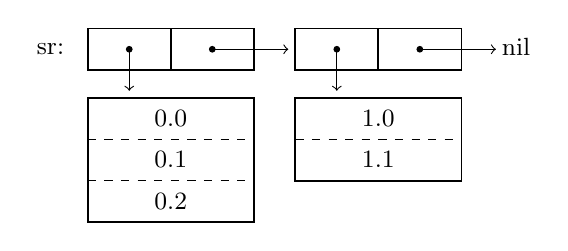
\begin{tikzpicture}
  \tikzstyle{every node}=[font=\small]

% список
  \draw (-0.5em, -0.75em) node[left] {\ic{sr}:};

  \draw [semithick] (0.0em, 0.0em) rectangle (6.0em, -1.5em);
  \draw [semithick] (3.0em, 0.0em) -- (3.0em, -1.5em);

  \filldraw  (4.5em, -0.75em) circle(1.0pt);
  \draw [->] (4.5em, -0.75em) -- (7.25em, -0.75em);

  \draw [semithick] (7.5em, 0.0em) rectangle (13.5em, -1.5em);
  \draw [semithick] (10.5em, 0.0em) -- (10.5em, -1.5em);

  \filldraw  (12.0em, -0.75em) circle(1.0pt);
  \draw [->] (12.0em, -0.75em) -- (14.75em, -0.75em);

  \draw [semithick] (14.6em, -0.65em) node[right] {\ii{nil}};

% окружения
  \filldraw  (1.5em, -0.75em) circle(1.0pt);
  \draw [->] (1.5em, -0.75em) -- (1.5em, -2.25em);
  \draw [semithick] (0.0em, -2.5em) rectangle (6.0em, -7.0em);
  \draw             (3.0em, -2.6em) node[below] {\ic{0.0}};
  \draw [dashed]    (0.0em, -4.0em) -- (6.0em, -4.0em);
  \draw             (3.0em, -4.1em) node[below] {\ic{0.1}};
  \draw [dashed]    (0.0em, -5.5em) -- (6.0em, -5.5em);
  \draw             (3.0em, -5.6em) node[below] {\ic{0.2}};

  \filldraw  (9.0em, -0.75em) circle(1.0pt);
  \draw [->] (9.0em, -0.75em) -- (9.0em, -2.25em);
  \draw [semithick] ( 7.5em, -2.5em) rectangle (13.5em, -5.5em);
  \draw             (10.5em, -2.6em) node[below] {\ic{1.0}};
  \draw [dashed]    ( 7.5em, -4.0em) -- (13.5em, -4.0em);
  \draw             (10.5em, -4.1em) node[below] {\ic{1.1}};

\end{tikzpicture}

\end{center}%
\caption{Окружение как список записей активаций.}%
\label{fast/fast/activations/fig:env-lists}%
\end{figure}

Можно сделать ещё лучше, введя специальное поле, с~помощью которого записи
активаций будут связываться в~список. Так как время на выделение памяти
в~среднем слабо зависит от размера объекта (если закрыть глаза на
инициализацию), то выделить память для одной записи активации с~лишним полем
выходит быстрее, чем для записи активации и точечной пары отдельно. Так и
поступим (рисунок~\ref{fast/fast/activations/fig:env-linked}), сделав подобное
поле первым, чтобы его расположение не~зависело от количества хранимых в~записи
переменных.

\indexC{activation-frame}
\indexC{environment}
\begin{code:lisp}
(define-class environment Object
  ( next ) )

(define-class activation-frame environment
  ( (* argument) ) )
\end{code:lisp}

\indexR{лексическое окружение}
\indexR{окружение!лексическое}
Значения, образующие лексическое окружение, хранятся в~связном списке записей
активаций. Функция \ic{sr-extend*} позволяет добавить в~окружение новую запись:

\indexC{sr-extend*}
\begin{code:lisp}
(define (sr-extend* sr v*)
  (set-environment-next! v* sr)
  v* )
\end{code:lisp}

Как видите, записи активаций физически модифицируются при расширении окружения,
так что функции не~могут разделять их между собой. Каждый вызов функции создаёт
собственные привязки, а значит, новую запись активации.

\indexR{адрес переменной}
\indexR{переменные!адреса}
Теперь вспомним, как представляются лексические окружения в~денотационном
интерпретаторе: они состоят из двух отдельных частей: $\rho$~и~$\sigma$.
Окружение~$\rho$ связывает имена переменных с~адресами их значений
в~памяти~$\sigma$. Но у~нас сейчас практически не~осталось памяти как таковой.
Адресом переменной является её положение в~цепочке записей активаций, которое
описывается двумя числами: номером записи активации и индексом переменной в~ней.
Следующие две функции определяют чтение и модификацию таких переменных.

\indexC{deep-fetch}
\indexC{deep-update"!}
\begin{code:lisp}
(define (deep-fetch sr i j)
  (if (= i 0)
      (activation-frame-argument sr j)
      (deep-fetch (environment-next sr) (- i 1) j) ) )

(define (deep-update! sr i j v)
  (if (= i 0)
      (set-activation-frame-argument! sr j v)
      (deep-update! (environment-next sr) (- i 1) j v) ) )
\end{code:lisp}

\begin{figure}[ht]\begin{center}
% -*- coding: utf-8 -*-
% Окружение как непосредственный связный список
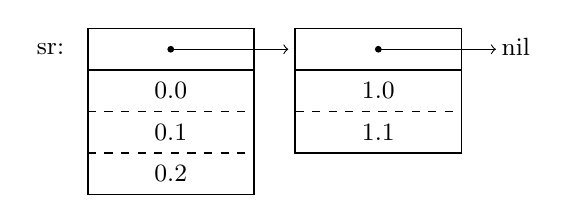
\begin{tikzpicture}
  \tikzstyle{every node}=[font=\small]

% список
  \draw (-0.5em, -0.75em) node[left] {\ic{sr}:};

  \draw [semithick] (0.0em, 0.0em) rectangle (6.0em, -6.0em);

  \filldraw  (3.0em, -0.75em) circle(1.0pt);
  \draw [->] (3.0em, -0.75em) -- (7.25em, -0.75em);

  \draw [semithick] (7.5em, 0.0em) rectangle (13.5em, -4.5em);

  \filldraw  (10.5em, -0.75em) circle(1.0pt);
  \draw [->] (10.5em, -0.75em) -- (14.75em, -0.75em);

  \draw (14.6em, -0.65em) node[right] {\ii{nil}};

% окружения
  \draw (0.0em, -1.5em) -- (6.0em, -1.5em);
  \draw          (3.0em, -1.6em) node[below] {\ic{0.0}};
  \draw [dashed] (0.0em, -3.0em) -- (6.0em, -3.0em);
  \draw          (3.0em, -3.1em) node[below] {\ic{0.1}};
  \draw [dashed] (0.0em, -4.5em) -- (6.0em, -4.5em);
  \draw          (3.0em, -4.6em) node[below] {\ic{0.2}};

  \draw (7.5em, -1.5em) -- (13.5em, -1.5em);
  \draw          (10.5em, -1.6em) node[below] {\ic{1.0}};
  \draw [dashed] ( 7.5em, -3.0em) -- (13.5em, -3.0em);
  \draw          (10.5em, -3.1em) node[below] {\ic{1.1}};

\end{tikzpicture}

\end{center}%
\caption{Окружение как непосредственно связный список.}%
\label{fast/fast/activations/fig:env-linked}%
\end{figure}

\indexE{r @\protect\ic{r} (лексическое окружение)}
\indexE{s r@\protect\ic{sr} (записи активаций)}
\indexR{лексические индексы}
\indexR{индексы!лексические}
Записи активаций представляют связи между адресами и значениями, а окружения
"--- между именами и адресами переменных. Поэтом теперь память (от~прямой
манипуляции которой мы хотим избавиться) фактически хранит исключительно записи
активаций. Окружения по аналогии с~$\rho$ мы будем называть~\ic{r}. Память
является \emph{состоянием} всех окружений, поэтому она именуется~\ic{sr}. Сами
окружения, по-хорошему, стоило~бы представлять подобно памяти, но знакомые вам
<<гирлянды>> из списков \seeEx[basics/ex:new-extend] являются вполне приемлемым
вариантом. Окружения расширяются функцией \ic{r-extend*} (не~путать
с~\ic{sr-extend*}); кроме неё нам потребуется <<полупредикат>>
\ic{local-variable?}, возвращающий \term{лексические индексы} переменных.

\indexC{r-extend*}
\indexC{local-variable"?}
\begin{code:lisp}
(define (r-extend* r n*)
  (cons n* r) )

(define (local-variable? r i n)
  (and (pair? r)
       (let scan ((names (car r))
                  (j 0) )
         (cond ((pair? names)
                (if (eq? n (car names))
                    `(local ,i . ,j)
                    (scan (cdr names) (+ 1 j)) ) )
               ((null? names)
                (local-variable? (cdr r) (+ i 1) n) )
               ((eq? n names) `(local ,i . ,j)) ) ) ) )
\end{code:lisp}

Всё это сделано для того, чтобы привести структуру памяти к~строго
иерархическому виду. Сейчас адрес переменной "--- это не~абсолютный номер ячейки
памяти, а пара \emph{относительных} координат в~текущем списке записей
активаций. Таким образом, сами адреса являются статическими и могут мигрировать
на этапе предварительной обработки, а значения переменных определяются как
обычно: динамически с~помощью адресов и текущего состояния памяти.

Подобное разделение лексического окружения на статическую и динамическую части
не~зависит от реализации памяти. На самом деле, это глубинное свойство самих
лексических окружений, которое стало явным только сейчас. Реализация памяти
в~денотационном интерпретаторе тоже позволяет предсказывать <<положение>>
значения переменной в~памяти (считая положением количество сравнений адресов
при поиске) по окружению, так как окружения представляются цепочками замыканий
вида \ic{(lambda (u) (if (eq? u~\ii{x}) \ii{y} (\ii{f}~u)))}.


\subsection{Интерпретатор: начало}\label{fast/fast/ssect:begin}

Сейчас мы уже знаем достаточно для того, чтобы набросать ядро интерпретатора и
реализовать несколько специальных форм. Ожидаемо, начнём мы работу с~функции
\ic{meaning}, имеющей следующий~тип:
%
\begin{multline*}
\text{\ic{meaning}:} \quad
  \underbrace{\Vset{Программа} \times
            \Vset{Окружение}}_{\text{статическая часть}}\to{} \\
  {} \to \underbrace{(\Vset{ЗаписиАктиваций}^* \times
            \Vset{Продолжение} \to \Vset{Значение})}_{\text{динамическая часть}}
\end{multline*}

\indexR{предобработка программ}
Здесь чётко видно, как именно лексические окружения разделяются на две части:
статические привязки имён к~адресам в~\Vset{Окружениях} и динамические привязки
адресов к~значениям в~\Vset{ЗаписяхАктиваций}. Программа, прошедшая подобную
\term{предобработку}, превращается в~функцию, ожидающую связный список записей
активаций (состояние памяти) и продолжение для того, чтобы вычислить результат.
Такой необычный способ представления программ весьма далёк от изначальных
S"=выражений, но принципиально остаётся тем~же.

\indexR{соглашения именования}
\indexE{e @\protect\ic{e} (выражения)}
\indexE{r @\protect\ic{r} (лексическое окружение)}
\indexE{s r@\protect\ic{sr} (записи активаций)}
\indexE{k @\protect\ic{k} (продолжения)}
\indexE{v @\protect\ic{v} (значения)}
\indexE{f @\protect\ic{f} (функции)}
\indexE{n @\protect\ic{n} (идентификаторы)}
Как обычно, ради упрощения синтаксического анализа разбираемые программы
считаются синтаксически корректными. Вспомним наши соглашения именования
сущностей:
 
\begin{center}\begin{tabular}{rl}
          \ic{e} & выражения, формы  \\
          \ic{r} & окружения         \\
\ic{sr}, \ic{v*} & записи активаций  \\
 \ic{k}, \ic{kk} & продолжения       \\
          \ic{v} & значения          \\
          \ic{f} & функции           \\
          \ic{n} & идентификаторы
\end{tabular}\end{center}

Отлично, вот синтаксический анализатор:

\indexC{meaning}
\begin{code:lisp}
(define (meaning e r)
  (if (atom? e)
      (if (symbol? e) (meaning-reference e r)
                      (meaning-quotation e r) )
      (case (car e)
        ((quote)  (meaning-quotation (cadr e) r))
        ((lambda) (meaning-abstraction (cadr e) (cddr e) r))
        ((if)     (meaning-alternative (cadr e) (caddr e) (cadddr e) r))
        ((begin)  (meaning-sequence (cdr e) r))
        ((set!)   (meaning-assignment (cadr e) (caddr e) r))
        (else     (meaning-application (car e) (cdr e) r)) ) ) )
\end{code:lisp}

Цитирование в~этот раз тривиально:

\indexC{meaning-quotation}
\begin{code:lisp}
(define (meaning-quotation v r)
  (lambda (sr k)
    (k v) ) )
\end{code:lisp}

\ForLayout{display}{\begingroup
\lstset{aboveskip=\smallskipamount, belowskip=\smallskipamount}}

Ветвление показывает хороший пример миграции кода. Предварительную обработку
проходят обе ветки независимо от того, какая из них будет выбрана
в~действительности.

\indexC{meaning-alternative}
\begin{code:lisp}
(define (meaning-alternative e1 e2 e3 r)
  (let ((m1 (meaning e1 r))
        (m2 (meaning e2 r))
        (m3 (meaning e3 r)) )
    (lambda (sr k)
      (m1 sr (lambda (v)
               ((if v m2 m3) sr k) )) ) ) )
\end{code:lisp}

Упорядочиваются формы как обычно, с~помощью рассмотрения двух возможных
вариантов списка~форм.

\indexC{meaning-sequence}
\begin{code:lisp}
(define (meaning-sequence e+ r)
  (if (pair? e+)
      (if (pair? (cdr e+))
          (meaning*-multiple-sequence (car e+) (cdr e+) r)
          (meaning*-single-sequence (car e+) r) )
      (static-wrong "Illegal syntax: (begin)") ) )

(define (meaning*-single-sequence e r)
  (meaning e r) )

(define (meaning*-multiple-sequence e e+ r)
  (let ((m1 (meaning e r))
        (m+ (meaning-sequence e+ r)) )
    (lambda (sr k)
      (m1 sr (lambda (v)
               (m+ sr k) )) ) ) )
\end{code:lisp}

Сложности начинаются с~аппликацией. Для неё нам придётся точнее описать протокол
вызова функций.


\subsubsection{Аппликация}\label{fast/fast/begin/ssect:application}

\indexR{протокол вызова функций}
\indexR{функции!протокол вызова}
Для обработки аппликаций необходимо определить несколько вещей: как выделяется
память под аргументы, как она заполняется и как передаётся, "--- короче говоря,
как используются записи активаций. Предварительная обработка функционального
терма аппликации проблем не~представляет, аргументы требуют чуть больше
внимания, так что для их обработки мы введём функцию \ic{meaning*}. Наконец,
тела функций для простоты реализуются с~помощью родных замыканий Scheme.

\indexC{meaning-regular-application}
\begin{code:lisp}
(define (meaning-regular-application e e* r)
  (let* ((m (meaning e r))
         (m* (meaning* e* r (length e*))) )
    (lambda (sr k)
      (m sr (lambda (f)
              (if (procedure? f)
                  (m* sr (lambda (v*) (f v* k)))
                  (wrong "Not a function" f) ) )) ) ) )
\end{code:lisp}

\ForLayout{display}{\endgroup}% \lstset *skipamount

\phantomlabel{fast/fast/begin/application/par:call/cc}
\indexR{записи активации!момент создания}
В~наших интересах выполнить как можно больше вычислений на этапе предобработки.%
\footnote*{Именно ради этого разработчики языков программирования стараются
сделать как можно больше вещей доступными статически.} Например, определить
размер необходимой записи активации. Сейчас это сделать элементарно, зная длину
списка аргументов. В~противоположность этому, гораздо сложнее сказать,
\emph{когда} создавать запись. Есть два возможных момента времени:

\begin{enumerate}
  \item Создавать запись активации до вычисления аргументов. В~этом
        случае вычисленные аргументы кладутся сразу~же на нужное место.

  \item Создавать запись активации после вычисления всех аргументов.
        В~таком случае, конечно~же, аргументы надо будет где"~то хранить
        до того, как они будут размещены в~нужной записи активации.
\end{enumerate}

\phantomlabel{fast/fast/begin/application/par:act-rec-before}
\indexR{записи активации!и call/cc@и~\protect\ic{call/cc}}
\indexR{продолжения (continuations)!множественные возвраты}
\indexR{возвращаемые значения!многократно}
Первый вариант кажется более эффективным, так как потребляет меньше памяти.
К~сожалению, в~Scheme есть \ic{call/cc}, из"~за которой этот вариант может
работать неверно. Он работает правильно только в~Лиспе. Причина лежит в~том,
что неограниченные продолжения Scheme можно активировать несколько раз.
\seePage[escape/forms/immortal/par:reincarnate] Если сначала создать запись
активации для вызываемой функции, а потом в~процессе вычисления её аргументов
захватить продолжение, то все параллельные активации данного продолжения будут
пользоваться физически одной и той~же записью, "--- а~ведь каждый вызов функции
должен иметь свою собственную. Для пояснения проблемы рассмотрим следующий
пример. Ожидается, что эта программа вернёт \ic{(2~1)}, но фактически она
возвращает \ic{(2~2)} в~случае разделяемых записей активаций.\footnote*{%
Мануэль~Серрано (Manuel~Serrano) обнаружил, что данная программа зависит от
порядка вычисления аргументов: форма \ic{cons} должна вычисляться слева направо.
Поэтому и используется \ic{let}.} Дело в~том, что \ic{call/cc} захватывает
аппликацию \ic{((lambda (a) ...) ...)} и её запись активации, если она была
создана заранее. Так как продолжение используется дважды, то оба созданных
замыкания \ic{(lambda () a)} ссылаются на физически одну и ту~же
переменную~\ic{a}, а~значит, активация продолжения \ic{(k~2)} сделает её
(в~обоих местах) равной~двум.

\begin{code:lisp}
(let ((k 'wait)
      (f '()) )
  (set! f (let ((g ((lambda (a) (lambda () a))
                    (call/cc (lambda (nk) (set! k nk) (nk 1))) )))
            (cons g f) ))
  ;; $\text{\ic{f}} \approx \text{\ic{(list $\lambda.$1)}}$
  (if (null? (cdr f)) (k 2))
  ;; $\text{\ic{f}} \approx \text{\ic{(list $\lambda.$2 $\lambda.$1)}}$
  (list ((car f)) ((cadr f))) )
\end{code:lisp}

\indexC{call/cc}
Но ещё не~всё потеряно! Записи активаций можно эффективно создавать до
вычисления аргументов функции, но тогда \ic{call/cc} придётся самостоятельно
делать копии записей активаций при каждой активации продолжения. К~сожалению,
сейчас она не~может этого делать вообще, так как продолжения представляются
родными замыканиями языка реализации и извлечь замкнутые в~них записи нельзя.
Вот ещё один пример того, насколько сильно \ic{call/cc} влияет на~реализацию.

Таким образом, функция \ic{meaning*} принимает дополнительный аргумент,
указывающий размер необходимой записи активации, которая будет создана после
вычисления всех аргументов. \seeEx[fast/ex:act-rec-before] По причинам, которые
будут разобраны в~разделе~\ref{fast/fast/ssest:varargs} вместе с~реализацией
функций переменной арности \seePage[fast/fast/ssest:varargs], записи активаций
получают на одно поле больше, чем надо обычным функциям, но это не~повлияет на
их эффективность, так как данное поле не~инициализируется.

\indexC{meaning*}
\indexC{meaning-no-arguments}
\begin{code:lisp}
(define (meaning* e* r size)
  (if (pair? e*)
      (meaning-some-arguments (car e*) (cdr e*) r size)
      (meaning-no-arguments r size) ) )

(define (meaning-no-arguments r size)
  (let ((size+1 (+ size 1)))
    (lambda (sr k)
      (let ((v* (allocate-activation-frame size+1)))
        (k v*) ) ) ) )
\end{code:lisp}

Заметьте, что \ic{size+1} вычисляется во~время предобработки "--- это значение
неизменно во~время исполнения, поэтому его можно вычислить сразу~же. Также
обратите внимание на <<оседлость>> формы, создающей запись активации: она
действительно должна вызываться при каждой аппликации.

Будущее расположение аргументов в~записи активации легко вычисляется заранее,
так что значение каждого аргумента после создания записи тут~же укладывается
в~свою забронированную ячейку.

\indexC{meaning-some-arguments}
\begin{code:lisp}
(define (meaning-some-arguments e e* r size)
  (let ((m (meaning e r))
        (m* (meaning* e* r size))
        (index (- size (+ (length e*) 1))) )
    (lambda (sr k)
      (m sr (lambda (v)
              (m* sr (lambda (v*)
                       (set-activation-frame-argument! v* index v)
                       (k v*) )) )) ) ) )
\end{code:lisp}

Вот теперь мы, наконец, можем определить абстракцию, в~точности зная, что
происходит с~аргументами. Для проверки арности используется длина записи
активации, но правильное значение известно заранее, а фактическое к~моменту
вызова функции уже вычислено и размещено по известному смещению, так что сейчас
нам остаётся только сравнить два готовых числа.

\indexC{meaning-fix-abstraction}
\begin{code:lisp}
(define (meaning-fix-abstraction n* e+ r)
  (let* ((arity (length n*))
         (arity+1 (+ 1 arity))
         (r2 (r-extend* r n*))
         (m+ (meaning-sequence e+ r2)) )
    (lambda (sr k)
      (k (lambda (v* k1)
           (if (= (activation-frame-argument-length v*) arity+1)
               (m+ (sr-extend* sr v*) k1)
               (wrong "Incorrect arity") ) )) ) ) )
\end{code:lisp}


\subsection{Классы переменных}\label{fast/fast/ssest:classify}

\indexR{переменные!классификация}
Предыдущими определениями поддерживаются только локальные переменные, то~есть
переменные внутри \ic{lambda}-форм. Но ведь ещё остались глобальные переменные,
а~среди них "--- предопределённые \hbox{и/или} неизменяемые вроде \ic{cons} или
\ic{car}. Сейчас возможно их поместить разве что в~самую дальнюю запись
активации, но вы представляете, какой тогда будет скорость доступа к~ним.
Поэтому мы воспользуемся возможностью статически классифицировать переменные.

\indexC{g.current}
\indexC{g.init}
\indexR{дескрипторы!переменных}
Пусть глобальная переменная \ic{g.current} содержит список изменяемых глобальных
переменных обрабатываемой программы, а переменная \ic{g.init} "--- фиксированный
список предопределённых неизменяемых переменных: \ic{cons}, \ic{car} {\itd}
Функция \ic{compute-kind} определяет класс переменной и возвращает
соответствующий дескриптор.

\indexC{compute-kind}
\indexC{global-variable"?}
\begin{code:lisp}
(define (compute-kind r n)
  (or (local-variable? r 0 n)
      (global-variable? g.current n)
      (global-variable? g.init n) ) )

(define (global-variable? g n)
  (let ((var (assq n g)))
    (and (pair? var) (cdr var)) ) )
\end{code:lisp}

\phantomlabel{fast/fast/classify/par:redefine}
\indexR{предопределённые переменные!переопределение}
\ic{g.current} проверяется перед \ic{g.init}, чтобы оставить возможность при
необходимости <<переопределять>> предопределённые переменные. Естественно,
значения этих переменных нельзя и не~следует изменять, но стандартом допускается
возможность определения одноимённых глобальных переменных при условии, что это
не~повлияет на работу примитивов. То~есть можно определить, например, глобальную
переменную \ic{car}, но \ic{map}, которая наверняка использует функцию \ic{car},
должна продолжать работать по-старому. Только явно определяемые в~этой~же
программе функции смогут пользоваться новым значением предопределённой
переменной. Одной \ic{compute-kind} достаточно для использования готовых
переопределений, но для создания новых придётся ввести дополнительную
специальную форму, скажем, \ic{redefine}. \seeEx[fast/ex:redefine]

Создаются глобальные переменные с~помощью функций \ic{g.init-extend!}
и~\ic{g.current-extend!}.

\indexC{g.current-extend"!}
\indexC{g.init-extend"!}
\begin{code:lisp}
(define (g.current-extend! n)
  (let ((level (length g.current)))
    (set! g.current (cons (cons n `(global . ,level)) g.current))
    level ) )

(define (g.init-extend! n)
  (let ((level (length g.init)))
    (set! g.init (cons (cons n `(predefined . ,level)) g.init))
    level ) )
\end{code:lisp}

Окружения \ic{g.current} и \ic{g.init} содержат лишь адреса, собственно значения
будут располагаться в~специально отведённом месте для глобальных переменных "---
двух векторах, доступных посредством переменных \ic{sg.current} и \ic{sg.init}.
Префикс~\ic{s} здесь потому, что данные векторы "--- это всё~же кусочек памяти.
Теперь определим эти контейнеры\footnote{Для простоты количество глобальных
переменных пока что ограничено одной сотней. Данное ограничение будет снято
в~разделе~\ref{fast/fast/ssect:variations}.} и функции-аксессоры к~ним.
(Конечно, без \ic{predefined-update!}, так как примитивы неизменяемы.)

\indexC{sg.current}
\indexC{sg.init}
\indexC{global-fetch}
\indexC{global-update"!}
\indexC{predefined-fetch}
\begin{code:lisp}
(define sg.current (make-vector 100))
(define sg.init (make-vector 100))

(define (global-fetch i)     (vector-ref sg.current i))
(define (predefined-fetch i) (vector-ref sg.init i))
(define (global-update! i v) (vector-set! sg.current i v))
\end{code:lisp}

Как обычно, мы определим пару вспомогательных функций \ic{g.current-initialize!}
и \ic{g.init-initialize!}, чтобы облегчить наполнение глобальных окружений.
Они будут синхронно обновлять глобальные окружения, следя за тем, чтобы
определяемая переменная (изначально) находилась только в~одном из~них.

\indexC{g.current-initialize"!}
\indexC{g.init-initialize"!}
\begin{code:lisp}
(define (g.current-initialize! name)
  (let ((kind (compute-kind r.init name)))
    (if kind
        (case (car kind)
          ((global)
           (vector-set! sg.current (cdr kind) undefined-value) )
          (else (static-wrong "Wrong redefinition" name)) )
        (let ((index (g.current-extend! name)))
          (vector-set! sg.current index undefined-value) ) ) )
  name )

(define (g.init-initialize! name value)
  (let ((kind (compute-kind r.init name)))
    (if kind
        (case (car kind)
          ((predefined) (vector-set! sg.init (cdr kind) value))
          (else (static-wrong "Wrong redefinition" name)) )
        (let ((index (g.init-extend! name)))
          (vector-set! sg.init index value) ) ) )
  name )
\end{code:lisp}


\indexR{предопределённые переменные!встраивание}
\indexR{встраивание!предопределённых переменных}
\indexR{переменные!предопределённые}
Теперь у~нас есть полный арсенал функций для реализации предварительной
обработки обращений к~переменным и присваиваний. Оба обработчика имеют весьма
схожую структуру: выяснить класс переменной и подать правильный аксессор.
Заметьте, что функции \ic{deep-fetch} и \ic{deep-update!} не~используются, если
переменная находится на верхушке стека записей активаций "--- в~этом случае
значения получаются и изменяются напрямую. Также здесь применяется одна
искусная, но спорная уловка: предопределённые переменные считаются чем"~то вроде
цитат: обращения к~ним сразу~же заменяются соответствующими значениями, а
не~выполняют вызовы аксессоров.

\indexC{meaning-reference}
\begin{code:lisp}
(define (meaning-reference n r)
  (let ((kind (compute-kind r n)))
    (if kind
        (case (car kind)
          ((local)
           (let ((i (cadr kind))
                 (j (cddr kind)) )
             (if (= i 0)
                 (lambda (sr k)
                   (k (activation-frame-argument sr j)) )
                 (lambda (sr k)
                   (k (deep-fetch sr i j)) ) ) ) )
          ((global)
           (let ((i (cdr kind)))
             (if (eq? (global-fetch i) undefined-value)
                 (lambda (sr k)
                   (let ((v (global-fetch i)))
                     (if (eq? v undefined-value)
                         (wrong "Uninitialized variable" n)
                         (k v) ) ) )
                 (lambda (sr k)
                   (k (global-fetch i)) ) ) ) )
          ((predefined)
           (let* ((i (cdr kind))
                  (value (predefined-fetch i)) )
             (lambda (sr k) (k value)) ) ) )
        (static-wrong "No such variable" n) ) ) )
\end{code:lisp}

Присваивание аналогично:

\indexC{meaning-assignment}
\begin{code:lisp}
(define (meaning-assignment n e r)
  (let ((m (meaning e r))
        (kind (compute-kind r n)) )
    (if kind
        (case (car kind)
          ((local)
           (let ((i (cadr kind))
                 (j (cddr kind)) )
             (if (= i 0)
                 (lambda (sr k)
                   (m sr (lambda (v)
                           (k (set-activation-frame-argument!
                               sr j v )) )) )
                 (lambda (sr k)
                   (m sr (lambda (v)
                           (k (deep-update! sr i j v)) )) ) ) ) )
          ((global)
           (let ((i (cdr kind)))
             (lambda (sr k)
               (m sr (lambda (v)
                       (k (global-update! i v)) )) ) ) )
          ((predefined)
           (static-wrong "Immutable predefined variable" n) ) )
        (static-wrong "No such variable" n) ) ) )
\end{code:lisp}


\subsubsection{Статические ошибки}\label{fast/fast/classify/sssect:static-err}

\indexR{ошибки!статические}
\indexR{ошибки!динамические}
Одна из целей предварительной обработки программ "--- это заранее отыскать все
глупые ошибки вроде обращений к~явно несуществующим переменным или попыток
изменения значений предопределённых переменных. Ведь без обработки они остаются
незамеченными, пока ошибочный код не~вызывается. О~таких ошибках сигнализирует
форма \ic{static-wrong}, тогда как \ic{wrong} служит для ошибок времени
исполнения, которые нельзя предвидеть заранее. Идея статических ошибок (ошибок
времени компиляции) очень полезна, но в~то~же время проводит чёткую границу
между либеральными языками вроде Лиспа и большей частью остальных. К~примеру,
любая корректная программа на~ML гарантированно лишена ошибок типизации.
В~Лиспе~же всё наоборот: только гарантированно ошибочные программы считаются
некорректными. Рассмотрим следующую функцию:

\indexC{fact}
\begin{code:lisp}
(define (statically-strange n)
  (if (integer? n)
      (if (= n 0) 1 (* n (statically-strange (- n 1))))
      (cons) ) )
\end{code:lisp}

Несмотря на то, что статически (в~общем случае) эта функция ошибочна, она может
быть весьма полезной, если ей передавать целые числа (особенно положительные!).
Разрешать подобные определения или нет "--- это вопрос духа языка, это
компромисс между желаемой безопасностью и отдаваемой за неё свободой. Очевидно,
что о~возможных ошибках лучше быть извещённым как можно раньше "--- ML возводит
эту максиму в~абсолют, "--- однако, как показывает Лисп, вполне можно жить пусть
и с~постоянной опасностью ошибиться, но получая взамен неимоверную гибкость
языка.

\indexC{static-wrong}
Поэтому функция \ic{static-wrong} должна, конечно~же, сообщать об~ошибке, но при
этом обязана возвращать нормальный результат предобработки. Конечно, вся его
работа сводится к~сообщению о~том, что мы таки наступили на грабли.
Предупреждение можно вывести заранее, но \emph{возникнуть} ошибка может только
во~время исполнения программы. Мы явно описываем желаемое поведение
в~определении \ic{static-wrong}:

\begin{code:lisp}
(define (static-wrong message . culprits)
  (display `(*static-error*
             ,message . ,culprits) )
  (newline)
  (lambda (sr k)
    (apply wrong message culprits) ) )
\end{code:lisp}

\noindent
Как говорится, и~рыбку съели, и~косточкой не~подавились.

\phantomlabel{fast/fast/classify/static-err/par:self-modify}
\indexR{глобальные переменные!инициализированность}
Кстати, вспомните, что при доступе к~глобальным переменным необходимо проверять
их инициализированность, чего не~требуется делать для~локальных и
предопределённых. Следовательно, есть некоторая дополнительная стоимость
обращения к~глобальным изменяемым переменным. В~случае компиляции на лету
(например, при выполнении чего"~то вроде \ic{(display (compile-and-run
(read)))}) мы могли~бы немного оптимизировать обращения к~инициализированным
глобальным переменным. В~действительности, у~нас даже сейчас есть подобная
оптимизация\footnote{Если~бы у~нас была возможность изменять скомпилированный
код на лету, то можно было~бы пойти и дальше: после инициализации переменной
просто выкинуть код проверок на инициализированность изо~всех обращений к~ней.
Например, так делает Bigloo~\cite{ser94}.} в~\ic{meaning-reference}.
\seeEx[compilation/ex:unchecked-ref]


\subsection{Запускаем интерпретатор}\label{fast/fast/ssest:starting}

Интерпретатор читает выражение, обрабатывает его, затем исполняет и повторяет
всё сначала. Таким образом, мы получаем компилирующий~REPL.

\indexC{chapter6.1-interpreter}
\begin{code:lisp}
(define  r.init '())
(define sr.init '())

(define (chapter6.1-interpreter)
  (define (compile e) (meaning e r.init))
  (define (run c) (c sr.init display))
  (define (toplevel)
    (run (compile (read)))
    (toplevel) )
  (toplevel) )
\end{code:lisp}

Конечно, перед его запуском стоит всё~же хоть немного наполнить базовое
окружение. Как обычно, предполагается, что у~нас есть готовые макросы,
которые выполнят всю чёрную рутинную работу, позволяя сфокусироваться на
главном. Вот несколько подобных определений; среди них, конечно~же, и наша
ненаглядная \ic{call/cc}.

\indexC{call/cc}
\begin{code:lisp}
(definitial t #t)
(definitial f #f)
(definitial nil '())

(defprimitive cons cons 2)
(defprimitive car car 1)

(definitial call/cc
  (let* ((arity 1)
         (arity+1 (+ 1 arity)) )
    (lambda (v* k)
      (if (= arity+1 (activation-frame-argument-length v*))
          ((activation-frame-argument v* 0)
           (let ((frame (allocate-activation-frame (+ 1 1))))
             (set-activation-frame-argument!
              frame 0
              (lambda (values kk)
                (if (= (activation-frame-argument-length values)
                       arity+1 )
                    (k (activation-frame-argument values 0))
                    (wrong "Incorrect arity" 'continuation) ) ) )
             frame )
           k )
          (wrong "Incorrect arity" 'call/cc) ) ) ) )
\end{code:lisp}


\subsection{Функции с~переменной~арностью}\label{fast/fast/ssest:varargs}

\indexR{функции!с переменной арностью}
\indexR{арность!переменная}
\indexR{переменная арность}
В~нашем интерпретаторе всё ещё не~поддерживаются функций с~переменной арностью.
Как всегда, реализация подобных функций представляет некоторые трудности. Наши
записи активаций хранят значения аргументов, но они~же фактически являются и
вместилищем привязок. Функции переменной арности нарушают правило <<один
аргумент "--- одна привязка>>. Например, функция, чьи аргументы описываются
списком \ic{(a b . c)}, может принять два, три, четыре или десять аргументов, но
привязок во~всех случаях будет ровно три. По этой причине в~записи активации
такой функции должно быть как минимум три поля. Аналогично для аппликации
\ic{(\ii{f} \ii{a} \ii{b})} тоже надо создавать запись активации с~тремя полями,
чтобы ей могла воспользоваться любая функция, которая может принять два
аргумента: то~есть функции со~списками аргументов вида \ic{(x~y)}, \ic{(x y .
z)}, \ic{(x~.~y)}, или даже просто~\ic{x}.

Соответственно, функции с~переменной арностью просто сбрасывают в~список все
<<лишние>> аргументы, которые они найдут в~записях активаций. Такую обработку
будет выполнять специально обученная функция \ic{listify!}. Она несложная, но,
требует определённой эквилибристики с~перераспределением переменных. Её параметр
\ic{arity} указывает минимальное количество принимаемых функцией аргументов.

\indexC{meaning-dotted-abstraction}
\indexC{listify"!}
\begin{code:lisp}
(define (meaning-dotted-abstraction n* n e+ r)
  (let* ((arity (length n*))
         (arity+1 (+ 1 arity))
         (r2 (r-extend* r (append n* (list n))))
         (m+ (meaning-sequence e+ r2)) )
    (lambda (sr k)
      (k (lambda (v* k1)
           (if (>= (activation-frame-argument-length v*) arity+1)
               (begin (listify! v* arity)
                      (m+ (sr-extend* sr v*) k1) )
               (wrong "Incorrect arity") ) )) ) ) )

(define (listify! v* arity)
  (let loop ((index (- (activation-frame-argument-length v*) 1))
             (result '()) )
    (if (= arity index)
        (set-activation-frame-argument! v* arity result)
        (loop (- index 1)
              (cons (activation-frame-argument v* (- index 1))
                    result ) ) ) ) )
\end{code:lisp}

Наконец, всё готово для предобработки обоих видов \ic{lambda}-форм. Выбор
необходимого обработчика легко выполняется статически:

\indexC{meaning-abstraction}
\begin{code:lisp}
(define (meaning-abstraction nn* e+ r)
  (let parse ((n* nn*)
              (regular '()) )
    (cond
     ((pair? n*) (parse (cdr n*) (cons (car n*) regular)))
     ((null? n*) (meaning-fix-abstraction nn* e+ r))
     (else (meaning-dotted-abstraction (reverse regular) n* e+ r)) ) ) )
\end{code:lisp}


\subsection{Приводимые выражения}\label{fast/fast/ssect:reducible}

\indexR{редексы}
\indexR{приводимые!формы}
\indexR{форма!приводимая}
\indexR{функции!переменной арности}
Давайте реализуем в~нашем интерпретаторе известную оптимизацию, касающуюся
приводимых форм (редексов): аппликаций, первым термом которых является
\ic{lambda}-форма. В~этом случае не~требуется создавать замыкание, достаточно
только ввести на время новые локальные переменные как в~блоках Алгола. В~конце
концов, \ic{((lambda (...) ...) ...)} "--- это не~что иное, как \ic{let}-форма:
всего лишь блок кода с~локальными переменными. И~снова, для функций
фиксированной арности всё легко и просто, чего не~скажешь об~арности
переменной.\footnote*{Это уже который раз мы такое говорим? Надеюсь, теперь вам
понятно, почему во~многих языках подобные функции не~реализованы вообще,
несмотря на всю их полезность.} Кстати, в~этом случае неправильное количество
аргументов является статически обнаруживаемой ошибкой.

\indexC{meaning-closed-application}
\indexC{meaning-fix-closed-application}
\begin{code:lisp}
(define (meaning-closed-application e ee* r)
  (let ((nn* (cadr e)))
    (let parse ((n* nn*)
                (e* ee*)
                (regular '()) )
      (cond ((pair? n*)
             (if (pair? e*)
                 (parse (cdr n*) (cdr e*) (cons (car n*) regular))
                 (static-wrong "Too few arguments" e ee*) ) )
            ((null? n*)
             (if (null? e*)
                 (meaning-fix-closed-application
                  nn* (cddr e) ee* r )
                 (static-wrong "Too many arguments" e ee*) ) )
            (else
             (meaning-dotted-closed-application
              (reverse regular) n* (cddr e) ee* r ) ) ) ) ) )

(define (meaning-fix-closed-application n* body e* r)
  (let* ((m* (meaning* e* r (length e*)))
         (r2 (r-extend* r n*))
         (m+ (meaning-sequence body r2)) )
    (lambda (sr k)
      (m* sr (lambda (v*)
               (m+ (sr-extend* sr v*) k) )) ) ) )
\end{code:lisp}

Для функций с~переменной арностью можно не~вызывать \ic{listify!}, так как
минимальная арность и фактическое число аргументов известны статически.
Специальный вариант \ic{meaning*}, названный \ic{meaning-dotted*}, отвечает за
обработку данного случая. Он работает подобно \ic{meaning*} для обязательных
аргументов, а дополнительные на лету собирает в~список, искусно расставляя
\ic{cons}. Конечно, это не~дёшево, но за удобства надо платить. Также придётся
вручную инициализировать последний элемент записи активации значением~\ic{()}.
В~общем, он выполняет вот такое преобразование:

{\def\a{$\alpha$}\def\b{$\beta$}\def\g{$\gamma$}\def\d{$\delta$}%
\def\E{\hbox to 0pt{\kern0.15em$\leadsto$}}
\begin{code:lisp}
((lambda (a b . c) ...) |\E|   ((lambda (a b c) ...)
 |\a| |\b| |\g| |\d| ...)               |\a| |\b| (cons |\g| (cons |\d| ...)) )
\end{code:lisp}}

\noindent
с~помощью вот таких функций:

\indexC{meaning-dotted-closed-application}
\indexC{meaning-dotted*}
\indexC{meaning-some-dotted-arguments}
\indexC{meaning-no-dotted-arguments}
\begin{code:lisp}
(define (meaning-dotted-closed-application n* n body e* r)
  (let* ((m* (meaning-dotted* e* r (length e*) (length n*)))
         (r2 (r-extend* r (append n* (list n))))
         (m+ (meaning-sequence body r2)) )
    (lambda (sr k)
      (m* sr (lambda (v*)
               (m+ (sr-extend* sr v*) k) )) ) ) )

(define (meaning-dotted* e* r size arity)
  (if (pair? e*)
      (meaning-some-dotted-arguments (car e*) (cdr e*) r size arity)
      (meaning-no-dotted-argument r size arity) ) )

(define (meaning-some-dotted-arguments e e* r size arity)
  (let ((m (meaning e r))
        (m* (meaning-dotted* e* r size arity))
        (index (- size (+ (length e*) 1))) )
    (if (< index arity)
        (lambda (sr k)
          (m sr (lambda (v)
                  (m* sr (lambda (v*)
                           (set-activation-frame-argument! v* index v)
                           (k v*) )) )) )
        (lambda (sr k)
          (m sr (lambda (v)
                  (m* sr (lambda (v*)
                           (set-activation-frame-argument!
                            v* arity
                            (cons v (activation-frame-argument
                                     v* arity )) )
                           (k v*) )) )) ) ) ) )

(define (meaning-no-dotted-argument r size arity)
  (let ((arity+1 (+ 1 arity)))
    (lambda (sr k)
      (let ((v* (allocate-activation-frame arity+1)))
        (set-activation-frame-argument! v* arity '())
        (k v*) ) ) ) )
\end{code:lisp}


\subsection{Интеграция примитивов}\label{fast/fast/ssect:integrating}

\indexR{примитивы}
\indexR{функции!примитивы}
Мы можем серьёзно ускорить интерпретацию, особым образом реализовав
предобработку вызовов примитивных предопределённых функций. Сейчас аппликация
вроде \ic{(car~$\alpha$)} вызывает ужасно расточительную кучу действий:

\begin{enumerate}
  \item Разыменовать глобальную переменную \ic{car}.

  \item Вычислить~$\alpha$.

  \item Создать запись активации с~двумя полями.

  \item Положить в~первое поле записи значение~$\alpha$.

  \item Убедиться, что значением \ic{car} действительно является
        функция.

  \item Убедиться, что эта функция действительно может принять
        один аргумент.

  \item Применить значение \ic{car} к~значению~$\alpha$. Вдобавок
        функция \ic{car} ещё проверяет, что её аргумент действительно
        является точечной парой.
\end{enumerate}

Некоторые из этих шагов не~нужны в~статически типизированных языках, именно
поэтому такие языки очень быстрые. Но при определённых усилиях можно избавиться
от некоторых проверок и в~Лиспе, выполняя их во~время предобработки. Так как
\ic{car} это глобальная переменная, чьё значение нельзя изменить, то мы
избавляемся от шага~5 (убедиться, что это функция) и шага~6 (проверить арность).
Можно сэкономить ещё больше, если не~создавать запись активации (шаги 3~и~4), а
сразу вставить код вызываемого примитива в~программу (шаг~1).

\phantomlabel{fast/fast/integrating/par:inlining}
\indexR{примитивы!встраивание}
\indexR{инлайнинг}
\indexR{встраивание}
\indexR{проверки типов}
\indexR{миграция!проверок типов}
Подобный способ использования примитивов "--- прямое исполнение кода в~обход
протокола вызова функций "--- называется \term{инлайнинг}. В~этом случае
остаётся выполнить только шаги 2~и~7. Вдобавок, хороший компилятор будет
выполнять седьмой шаг по-умному, избегая дублирования проверок типов. Например,
в~выражении \ic{(if (pair?~e) (car~e) ...)} бессмысленно проверять тип~\ic{e}
внутри \ic{car}, так как он очевидно и гарантированно правильный. Один из
способов реализации такого поведения следующий: считать \ic{(car~\ii{x})}
макросом, раскрывающимся в~\ic{(let ((\ii{v}~\ii{x})) (if (pair?~\ii{v})
(unsafe-car~\ii{v}) (error ...)))}, где \ic{unsafe-car}\footnote{Большинство
реализаций предоставляют подобные небезопасные примитивы, оказывающиеся весьма
полезными для различных преобразований программ. Естественно, эти преобразования
должны гарантировать использование \ic{unsafe}-примитивов только в~безопасном
контексте. Компилятор часто способен уследить за типами значений, хранимых
в~переменных, поэтому данные примитивы очень важны для эффективной компиляции.}
работает как \ic{car}, если её аргумент это точечная пара, и имеет
неопределённое поведение в~противном случае. Теперь остаётся только перенести
все проверки типов как можно выше, оставив таким образом лишь неизбежные и
избавившись от очевидных повторений. С~миграцией проверок типов проблем нет, так
как сами по себе они не~вызывают ошибок и бесконечных циклов.

\indexC{desc.init}
\indexR{дескрипторы!примитивов}
При настоящей компиляции мы не~имеем непосредственного доступа к~значениям
предопределённых переменных: они обычно лежат где"~то в~библиотеке времени
исполнения. Однако, для предварительной обработки программ эти значения
не~особо"~то и нужны, достаточно будет знать, функция~ли это и сколько
аргументов она может принять. Поэтому мы добавим новое окружение: окружение
дескрипторов глобальных предопределённых переменных \ic{desc.init}. В~нём будут
храниться описания предопределённых примитивных функций, представляемые
списками. Первый элемент такого списка "--- это символ \ic{function}, второй
"--- <<адрес>> примитива (то, что вызывается), а за ним следует описание
арности. Макрос \ic{defprimitive} используется для определения примитивов.
Здесь приведён только один из его подмакросов: \ic{defprimitive3}, определения
остальных аналогичны.

\indexC{defprimitive}
\begin{code:lisp}
(define-syntax defprimitive
  (syntax-rules ()
    ((defprimitive name value 0) (defprimitive0 name value))
    ((defprimitive name value 1) (defprimitive1 name value))
    ((defprimitive name value 2) (defprimitive2 name value))
    ((defprimitive name value 3) (defprimitive3 name value)) ) )

(define-syntax defprimitive3
  (syntax-rules ()
    ((defprimitive3 name value)
     (definitial name
       (letrec ((arity+1 (+ 3 1))
                (behavior
                 (lambda (v* k)
                   (if (= (activation-frame-argument-length v*)
                          arity+1 )
                       (k (value (activation-frame-argument v* 0)
                                 (activation-frame-argument v* 1)
                                 (activation-frame-argument v* 2) ))
                       (wrong "Incorrect arity" 'name) ) ) ) )
         (description-extend!
          'name `(function ,value a b c))
         behavior ) ) ) ) )
\end{code:lisp}

Управление новым окружением возлагается на следующие функции:

\indexC{description-extend"!}
\indexC{get-description}
\begin{code:lisp}
(define desc.init '())

(define (description-extend! name description)
  (set! desc.init (cons (cons name description) desc.init))
  name )

(define (get-description name)
  (let ((p (assq name desc.init)))
    (and (pair? p) (cdr p)) ) )
\end{code:lisp}

Вот теперь можно действительно полностью определить обработку аппликаций.
Она сводится к~определению класса вызываемой функции и передаче аппликации
соответствующему специфичному обработчику. Заметьте, что согласованность арности
для примитивов тоже проверяется статически.

\indexC{meaning-application}
\begin{code:lisp}
(define (meaning-application e e* r)
  (cond
   ((and (symbol? e)
         (let ((kind (compute-kind r e)))
           (and (pair? kind)
                (eq? 'predefined (car kind))
                (let ((desc (get-description e)))
                  (and desc
                       (eq? 'function (car desc))
                       (if (= (length (cddr desc)) (length e*))
                           (meaning-primitive-application e e* r)
                           (static-wrong "Incorrect arity" e) ) ) ) ) ) ))
   ((and (pair? e)
         (eq? 'lambda (car e)) )
    (meaning-closed-application e e* r) )
   (else (meaning-regular-application e e* r)) ) )
\end{code:lisp}

Аппликации примитивов обрабатываются следующим образом:

\indexC{meaning-primitive-application}
\begin{code:lisp}
(define (meaning-primitive-application e e* r)
  (let* ((desc (get-description e)) ; \ic{desc}${}={}$\ic{(function \ii{адрес} . \ii{аргументы})}
         (address (cadr desc))
         (size (length e*)) )
    (case size
     ((0) (lambda (sr k) (k (address))))
     ((1) (let ((m1 (meaning (car e*) r)))
            (lambda (sr k)
              (m1 sr (lambda (v)
                       (k (address v)) )) ) ))
     ((2) (let ((m1 (meaning (car e*) r))
                (m2 (meaning (cadr e*) r)) )
            (lambda (sr k)
              (m1 sr (lambda (v1)
                (m2 sr (lambda (v2)
                         (k (address v1 v2)) )) )) ) ))
     ((3) (let ((m1 (meaning (car e*) r))
                (m2 (meaning (cadr e*) r))
                (m3 (meaning (caddr e*) r)) )
            (lambda (sr k)
              (m1 sr (lambda (v1)
                (m2 sr (lambda (v2)
                  (m3 sr (lambda (v3)
                           (k (address v1 v2 v3)) )) )) )) ) ))
     (else (meaning-regular-application e e* r)) ) ) )
\end{code:lisp}

\indexR{примитивы!арность}
\indexR{арность!примитивов}
Данный вариант поддерживает только примитивы фиксированной арности. Большая
часть примитивов, обладающих переменной арностью, вроде \ic{append},
\ic{for-each}, \ic{list}, \ic{map}, \ic{*}, \ic{+} и~многие другие (но
не~\ic{apply}), могут считаться чем"~то вроде макросов: например, \ic{(append
$\pi_1$ $\pi_2$ $\pi_3$)} раскрывается в~\ic{(append $\pi_1$ (append $\pi_2$
$\pi_3$))}. Такая трансформация позволяет передавать произвольное число
аргументов, но спасает не~всегда. Например, в~случае \ic{(apply append $\pi$)}
примитивная функция \ic{append} уже вынуждена поддерживать произвольное число
аргументов самостоятельно.

Мы заменяем инлайн-версиями только аппликации с~тремя и менее аргументами.
Причина такого решения банальна: в~Scheme просто нет примитивных функций
с~фиксированной арностью, принимающих больше трёх аргументов!


\subsection{Вариации на~тему~окружений}\label{fast/fast/ssect:variations}

\indexR{свободные переменные!варианты реализации}
\indexR{дисплеи}
В~данный момент время доступа к~глубоко расположенным локальным переменным
(к~тем, которые не~находятся в~первой записи активации) линейно зависит от
их расположения, так как мы вынуждены каждый раз заново проходить по списку
записей активаций. Существует простой способ получать доступ ко~всем переменным
за постоянное время: поместить в~каждую запись активации \term{дисплей},
хранящий прямые ссылки на все записи, расположенные глубже
(см.~рисунок~\ref{fast/fast/variations/pic:display}). В~таком случае достаточно
будет одной косвенной адресации (через ячейку дисплея до записи) и одного сдвига
(до нужного значения в~индексированном поле записи). Ценой за повышение скорости
обращений является увеличение потребления памяти, а также замедление создания
новых записей активаций. Конечно, в~дисплее можно хранить ссылки не~на все
записи, а только на те, которые действительно используются, но это требует
соответствующего анализа всех обращений к~переменным. К~сожалению, мы не~можем
прямо воспользоваться этим приёмом в~нашем интерпретаторе, так как сейчас размер
записи активации фиксируется до вызова функции, а при использовании дисплеев он
будет известен только во~время исполнения. Необходимо или хранить дисплеи
отдельно от записей, или ограничить максимально возможную высоту стека (что
не~особо в~духе Лиспа).

\begin{figure}[!h]
\begin{center}
% -*- coding: utf-8 -*-
% Структура дисплеев
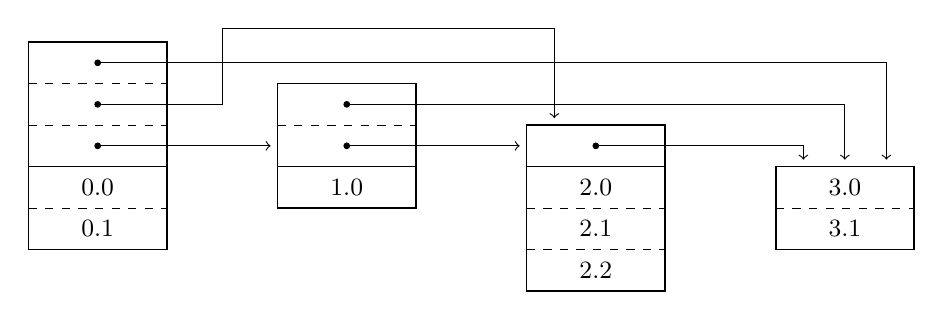
\begin{tikzpicture}
  \tikzstyle{every node}=[font=\small]

  \draw [semithick] (0.0em,  4.5em) rectangle (5.0em, -3.0em);
  \draw [dashed]    (0.0em,  3.0em) -- (5.0em, 3.0em);
  \draw [dashed]    (0.0em,  1.5em) -- (5.0em, 1.5em);
  \draw             (0.0em,  0.0em) -- (5.0em, 0.0em);
  \draw             (2.5em, -0.1em) node[below] {\ic{0.0}};
  \draw [dashed]    (0.0em, -1.5em) -- (5.0em, -1.5em);
  \draw             (2.5em, -1.6em) node[below] {\ic{0.1}};

  \draw [semithick] ( 9.0em,  3.0em) rectangle (14.0em, -1.5em);
  \draw [dashed]    ( 9.0em,  1.5em) -- (14.0em, 1.5em);
  \draw             ( 9.0em,  0.0em) -- (14.0em, 0.0em);
  \draw             (11.5em, -0.1em) node[below] {\ic{1.0}};

  \draw [semithick] (18.0em,  1.5em) rectangle (23.0em, -4.5em);
  \draw             (18.0em,  0.0em) -- (23.0em, 0.0em);
  \draw             (20.5em, -0.1em) node[below] {\ic{2.0}};
  \draw [dashed]    (18.0em, -1.5em) -- (23.0em, -1.5em);
  \draw             (20.5em, -1.6em) node[below] {\ic{2.1}};
  \draw [dashed]    (18.0em, -3.0em) -- (23.0em, -3.0em);
  \draw             (20.5em, -3.1em) node[below] {\ic{2.2}};

  \draw [semithick] (27.0em,  0.0em) rectangle (32.0em, -3.0em);
  \draw             (29.5em, -0.1em) node[below] {\ic{3.0}};
  \draw [dashed]    (27.0em, -1.5em) -- (32.0em, -1.5em);
  \draw             (29.5em, -1.6em) node[below] {\ic{3.1}};


  \filldraw  (2.5em, 3.75em) circle(1.0pt);
  \filldraw  (2.5em, 2.25em) circle(1.0pt);
  \filldraw  (2.5em, 0.75em) circle(1.0pt);
  \draw [->] (2.5em, 3.75em) -- (31.0em, 3.75em) -- (31.0em, 0.25em);
  \draw [->] (2.5em, 2.25em) -- (7.0em, 2.25em) -- (7.0em, 5.0em) --
               (19.0em, 5.0em) -- (19.0em, 1.75em);
  \draw [->] (2.5em, 0.75em) -- (8.75em, 0.75em);

  \filldraw  (11.5em, 2.25em) circle(1.0pt);
  \filldraw  (11.5em, 0.75em) circle(1.0pt);
  \draw [->] (11.5em, 2.25em) -- (29.5em, 2.25em) -- (29.5em, 0.25em);
  \draw [->] (11.5em, 0.75em) -- (17.75em, 0.75em);

  \filldraw  (20.5em, 0.75em) circle(1.0pt);
  \draw [->] (20.5em, 0.75em) -- (28.0em, 0.75em) -- (28.0em, 0.25em);

\end{tikzpicture}

\end{center}
\caption{Структура дисплеев.}\label{fast/fast/variations/pic:display}
\end{figure}


\subsubsection{Плоские окружения}\label{fast/fast/variations/ssect:flat}

\indexR{плоские окружения}
\indexR{окружение!плоское}
\indexR{коробки}
Другой вариант решения проблемы скорости доступа: избавиться от полноценного
стека окружений. Для каждого создаваемого замыкания можно не~просто слепо
сохранять внутри всё состояние окружения~\ic{sr}, а формировать для него
специальную запись активации, в~которой собираются все его свободные переменные.
В~этом случае, конечно, чуть возрастает стоимость создания замыканий, но все
свободные переменные будут доступны за постоянное время, так как в~окружениях
будет всего по две записи активации: одна с~собственными локальными переменными
активного замыкания, а другая "--- со~свободными. Конечно, на случай, если
потребуется разделять какую-либо переменную между несколькими замыканиями, имеет
смысл реализовать коробки. \seePage[assignment/assignment/boxes/p:boxing]

В~идеале, естественно, стоит использовать все возможные варианты, применяя
каждый из них в~тех случаях, для которых он работает лучше остальных. Чтобы
осуществлять такое адаптивное поведение, требуется более тщательный анализ
программ. Это работа для настоящего компилятора, а не~для простого
интерпретатора с~небольшой предобработкой вроде нашего.


\subsubsection{Определение глобальных~переменных}%
\label{fast/fast/variations/ssect:global-define}

\indexR{переменные!глобальные}
Наш интерпретатор считает, что переменная глобальная, если она находится
в~списке глобальных изменяемых или~же предопределённых переменных.
Следовательно, перед использованием переменную надо поместить в~один из этих
списков, иными словами: объявить. Внутри интерпретатора это выполняется
с~помощью макроса \ic{defvariable}:

\indexC{defvariable}
\begin{code:lisp}
(define-syntax defvariable
  (syntax-rules ()
    ((defvariable name)
     (g.current-initialize! 'name) ) ) )
\end{code:lisp}

\indexR{глобальные переменные!объявление}
Многие языки имеют что"~то подобное для явного объявления переменных, но
в~большинстве диалектов Лиспа принят другой подход. Здесь правильным считается
автоматическое создание всех используемых глобальных переменных. Один из
наиболее простых способов этого добиться: поместить механизм создания глобальных
переменных прямиком в~функцию \ic{compute-kind}:

\indexC{adjoin-global-variable"!}
\indexC{compute-kind}
\begin{code:lisp}
(define (compute-kind r n)
  (or (local-variable? r 0 n)
      (global-variable? g.current n)
      (global-variable? g.init n)
      [(adjoin-global-variable! n)] ) )

(define (adjoin-global-variable! name)
  (let ((index (g.current-extend! name)))
    (vector-set! sg.current index undefined-value)
    (cdr (car g.current)) ) )
\end{code:lisp}

\indexR{глобальные переменные!предрождение}
Но так делать не~совсем хорошо, потому что тогда предобработка берёт на себя
слишком много. Получается, что глобальные переменные создаются во~время неё, а
не~во~время исполнения программы. Приемлемо~ли такое предрождение? Давайте ещё
раз разберём, что именно происходит при упоминании новой переменной.

\begin{enumerate}
  \item Её имя добавляется в~окружение глобальных изменяемых переменных
        (известное как \ic{g.current}), а также с~переменной связывается
        уникальный номер.

  \item Для хранения значения переменной выделяется ячейка памяти
        с~адресом, соответствующим её~номеру.
\end{enumerate}

Держа это в~уме, рассмотрим следующую программу:

\begin{code:lisp}
(begin (define foo (lambda () (bar)))
       (define bar (lambda () (if #t 33 hux))) )
\end{code:lisp}

Так как в~процессе её предобработки были встречены неизвестные переменные
с~именами \ic{foo}, \ic{bar} и~\ic{hux}, то они все получают свои номера, ячейки
памяти и добавляются в~окружение. Но как их существование соотносится
с~семантикой обрабатываемой программы? Почему определение \ic{foo} игнорирует
явно заданный порядок вычисления форм? Зависит~ли существование \ic{hux} от
истинности условия?

Как~бы то~ни было, во~время исполнения программы значения всех используемых
глобальных переменных должны находиться в~глобальном окружении. Идеальный момент
для их добавления туда "--- это непосредственно перед началом исполнения
программы. Вернее, это единственно возможный момент. Лишь тогда размер
глобального окружения можно окончательно подогнать под требуемое количество
глобальных переменных, а также выдать им начальные значения. Это выполняет
функция \ic{standalone-producer}, которая обрабатывает программу, возвращая
обычное замыкание \ic{(lambda (sr k) ...)}, первым действием которого является
создание личного глобального окружения необходимых размеров.

\indexC{standalone-producer}
\begin{code:lisp}
(define (standalone-producer e)
  (set! g.current (original.g.current))
  (let* ((m (meaning e r.init))
         (size (length g.current)) )
    (lambda (sr k)
      (set! sg.current (make-vector size undefined-value))
      (m sr k) ) ) )
\end{code:lisp}

\indexC{original.g.current}
\indexR{переменные!предопределённые}
\indexR{предопределённые переменные!для общения с системой}
В~глобальном окружении могут быть и предопределённые изменяемые переменные,
служащие механизмом обмена информацией между программой и внешней системой. Они
могут содержать разнообразные настройки вроде основания счисления для вывода
чисел. Предполагается, что такие переменные содержатся в~окружении, возвращаемом
\ic{original.g.current}.

\indexR{глобальные переменные!объявление}
\indexE{Scheme!глобальные переменные}
Итого, при такой реализации для создания переменной достаточно лишь упомянуть
её имя. Можно было~бы поступить наоборот, как сделано в~Scheme, где глобальные
переменные создаются исключительно формой \ic{define}. В~этом случае
предобработка примера с~\ic{foo} должна выдать ошибку, так как \ic{hux} "---
это неопределённая переменная с~точки зрения предобработки, и не~важно, что
фактически к~ней никогда даже не~обратятся. Переменная \ic{bar} проблем
не~вызывает, так как её определение в~программе присутствует (пусть и чуть
дальше).

\ForLayout{display}{\begingroup
\lstset{aboveskip=\smallskipamount, belowskip=\smallskipamount}}

Для пояснения принципа работы \ic{define} мы добавим новую специальную форму
в~\ic{meaning}:

\begin{code:lisp}
... ((define) (meaning-define (cadr e) (caddr e) r)) ...
\end{code:lisp}

При обработке форм \ic{define} обнаруживаются все повторные определения
переменных. Хоть переопределение переменных не~является ошибкой, но лучше
предупредить пользователя. Так как все глобальные переменные уже будут
существовать перед выполнением программы, то все определения можно просто
заменять присваиваниями.

\indexC{meaning-define}
\begin{code:lisp}
(define (meaning-define n e r)
  (let ((b (memq n *defined*)))
    (if (pair? b)
        (static-wrong "Already defined variable" n)
        (set! *defined* (cons n *defined*)) ) )
  (meaning-assignment n e r) )
\end{code:lisp}

Также на предобработку возлагается дополнительная задача: проверить, все~ли
упоминаемые глобальные переменные были определены и получили значения.
Естественно, в~список определённых входят также и предопределённые переменные.

\indexC{set-difference}
\indexC{standalone-producer}
\begin{code:lisp}
(define (standalone-producer e)
  (set! g.current (original.g.current))
  (let ((originally-defined (append (map car g.current)
                                    (map car g.init) )))
    (set! *defined* originally-defined)
    (let* ((m (meaning e r.init))
           (size (length g.current))
           (anormals (set-difference (map car g.current) *defined*)) )
      (if (null? anormals)
          (lambda (sr k)
            (set! sg.current (make-vector size undefined-value))
            (m sr k) )
          (static-wrong "Undefined global variables" anormals) ) ) ) )

(define (set-difference set1 set2)
  (if (pair? set1)
      (if (memq (car set1) set2)
          (set-difference (cdr set1) set2)
          (cons (car set1) (set-difference (cdr set1) set2)) )
      '() ) )
\end{code:lisp}

\ForLayout{display}{\endgroup}% \lstset *skipamount

\indexCS{define}{семантика}
Подводя итог, необходимо чётко разделять предобработку и исполнение программ.
Во~время исполнения программы определения эквивалентны присваиваниям. Но
во~время предобработки они требуют больших усилий, проверок и так далее. Обычные
специальные формы (не~\ic{define}) действуют исключительно во~время исполнения
программ. Их семантика динамическая. Определение переменных "--- это статический
процесс (благодаря предобработке), потому как все глобальные переменные должны
быть определены с~помощью специальной формы \ic{define}, чьё наличие можно
проверить статически, а отсутствие считается ошибкой.

Кроме того, как мы упоминали ранее в~разговоре о~\ic{letrec}
\seePage[lisp1-2-omega/recusion/ssect:uninitialized], важно понимать, что
создание и инициализация переменных "--- это не~одно и то~же. Переменная может
существовать, но не~иметь при этом значения. Вот вам пример такой переменной:

\begin{code:lisp}
(begin (define foo bar)
       (define bar (lambda () 33)) )
\end{code:lisp}

В~случае компилирующего интерпретатора (нечто вроде инкрементального
компилятора, сразу~же вычисляющего скомпилированные им выражения) большая часть
рассмотренных проблем пропадает сама собой благодаря тому, что программа
выполняется сразу~же после её обработки и, что самое главное, с~тем состоянием
памяти, которое было на конец обработки. Поэтому здесь первый вариант
\ic{adjoin-global-variable!}, сразу~же добавляющий переменные в~память,
в~принципе подходит и работает правильно. То~же касается и улучшения
в~\ic{meaning-reference}, удаляющего проверки на инициализированность для уже
инициализированных переменных.


\subsection{Выводы: интерпретатор с~миграцией~вычислений}%
\label{fast/fast/ssect:conclusions}

Довольно сложно точно измерить достигнутое увеличение эффективности, но оно
составляет порядка 10"--~50 раз. Предварительная обработка выполняется
достаточно быстро, но возможности для оптимизации ещё остаются (самое очевидное:
представлять окружения не~списками, а хеш-таблицами). Кроме того, немаловажен и
новый подход с~разделением вычислений на статическую и динамическую части.
Хороший компилятор должен как можно больше всего выполнять статически, чтобы
во~время исполнения программа делала как можно меньше ненужных действий.
Естественно, непрестанно ведутся исследования, нацеленные на поиск новых
статических свойств программ, которые могли~бы улучшить качество
предварительной обработки. Вот лишь некоторые из них: абстрактная интерпретация
в~работе~\cite{cc77}, частичные вычисления из~\cite{jgs93}, анализ потока
исполнения в~\cite{shi91}. Ещё одним аспектом, влияющим на эффективность,
является выбор используемых структур данных, как можно было увидеть из нашей
дискуссии о~представлении записей активаций.

Предварительная обработка позволяет отловить некоторые ошибки заранее, до того,
как они возникнут при исполнении программы. Это первый шаг на пути к~более
безопасному и эффективному программированию: меньше возможных ошибок "--- меньше
явных проверок. Рассмотренная здесь обработка довольно примитивна, как минимум
её можно научить проверять типы, как это сделано в~ML.

Полученный интерпретатор очень напоминает рассмотренный в~третьей главе, разве
что замыкания в~нашем языке реализуются напрямую с~помощью родных замыканий
Scheme. Несмотря на то, что объекты и замыкания во~многом схожи, замыкания
всё~же недостаточно выразительны для данного случая: у~них только один метод
"--- вызов; их внутренняя структура покрыта мраком; их поведение невозможно
уточнить или изменить, не~говоря уже о~более сложных вещах вроде рефлексии.


\section{Отказ от~окружений}\label{fast/sect:reject}

\indexE{env@\protect\ic{*env*}}
Каждое выражение вычисляется в~так или иначе уникальном окружении, у~нас ему
соответствует значение параметра~\ic{sr}. Так как окружение изменяется
исключительно при вызовах функций "--- они восстанавливают окружение своего
создания, после чего расширяют его локальными переменными, "--- то, вероятно,
имеет смысл ввести явное понятие текущего состояния окружения, храня его
в~глобальной переменной (или регистре)~\ic{*env*}. Это позволило~бы избежать
передачи окружения через аргумент всем замыканиям, получающимся в~результате
предобработки. Иными словами, в~таком случае предварительная обработка будет
возвращать замыкания всего с~одним параметром: \ic{(lambda (k)~...)}.

На первый взгляд, для выполнения подобного преобразования, заменяющего локальные
переменные функций \ic{sr} одной глобальной переменной \ic{*env*}, достаточно
внести лишь косметические изменения:

\begin{enumerate}
  \item Отныне локальные переменные следует искать в~\ic{*env*},
        а не~в~\ic{sr}.

  \item Замыкания сохраняют расширенные окружения своего определения
        и при своём вызове просто устанавливают в~\ic{*env*} нужное им
        значение.
\end{enumerate}

\indexR{стек!вызовов}
\indexR{окружение!при вызовах функций}
\indexR{хвостовые вызовы}
\indexR{вызов!хвостовой}
Однако мы пропустили одну маленькую, но существенную деталь: время от времени
необходимо восстанавливать старое окружение, а именно, когда происходит возврат
к~вычислениям, прерванным вызовом функции. Решение в~лоб: функция при вызове
сохраняет текущее значение \ic{*env*}, а при возврате восстанавливает его. Но
вот здесь возникает проблема с~тем, что Scheme требует оптимизации хвостовых
вызовов, то~есть иногда \ic{*env*} восстанавливать \emph{не~надо}, потому что
хвостовые вызовы должны выполняться с~неизменным продолжением.

\indexR{протокол вызова функций}
\indexR{функции!протокол вызова}
Эта проблема напоминает проблему выбора протокола вызова функций на самом
низком, машинном уровне. При вызове необходимо сохранять и восстанавливать
регистры процессора, но кто это должен делать?

\begin{itemize}
  \item Вызываемая подпрограмма точно знает, какие регистры ей
        понадобятся, так что может сохранять только их. Сложность тут
        в~том, что восстановление регистров необходимо выполнять
        непосредственно перед возвратом управления из подпрограммы.
        Другими словам, это становится частью её продолжения.

  \item Вызывающий подпрограмму в~свою очередь знает, какие регистры
        понадобятся ему, поэтому может сохранить их самостоятельно.
        В~этом случае подпрограмма должна лишь выполниться и положить
        результат туда, где его ждут. Никаких проблем с~продолжениями,
        и если вызывающему не~важно состояние регистров, то можно вообще
        ничего не~делать. Правда, подпрограмме может быть нужна лишь пара
        регистров, но вызывающему об~этом она никак не~скажет.
\end{itemize}

\indexR{регистры!как стеки}
В~\cite{ss80} предлагается следующее решение: вызывающий помечает регистры
метками <<сохранить при использовании>> и <<можно свободно изменять>>, а
вызываемый может сохранять только то, что действительно надо сохранять, помечая
регистры как <<восстановить при возврате>> и <<значение не~менялось>>. Тогда
регистры становятся фактически стеками значений, где верхнее значение является
текущим, а под ним лежат дожидающиеся восстановления старые значения. Во~время
возврата управления специальная машинная инструкция обновляет значения регистров
в~соответствии с~расставленными метками.

Очень важно, чтобы хвостовые вызовы проводились с~неизменным продолжением
(то~есть не~вызывали роста стека), это позволяет эффективно реализовывать
итерацию через рекурсию, не~ограничивая возможную длину цикла размером стека.
Поэтому мы будем использовать вторую стратегию: ответственным за сохранение (или
несохранение) окружения является тот, кто вызывает функцию.

\indexC{tail"?}
К~счастью, найти все вызовы из хвостовых позиций можно статически, так что
функция \ic{meaning} получает дополнительный аргумент: булево значение
\ic{tail?}, показывающее, расположено~ли вычисляемое выражение в~хвостовой
позиции или нет. Если да, то можно не~восстанавливать окружение после завершения
вычислений. (Естественно, в~таком случае его и сохранять не~обязательно.)

\indexR{хвостовые вызовы!способ нахождения}
\indexR{вызов!хвостовой!способ нахождения}
Так где~же у~выражений хвост? Для ответа на этот вопрос следует обратиться
к~денотациям: всё, что вычисляется с~продолжением, отличным от продолжения
внешней формы, находится не~в~хвостовой позиции. В~присваивании \ic{(set! \ii{x}
$\pi$)} форма~$\pi$ имеет продолжение, отличное от такового у~формы \ic{set!},
так как ещё остаётся записать её значение в~переменную~\ii{x}. Следовательно,
это не~хвостовой вызов. Аналогично, форма~$\pi_0$ в~ветвлении \ic{(if $\pi_0$
$\pi_1$ $\pi_2$)} тоже не~является последним вычислением. В~последовательности
\ic{(begin $\pi_0$~... $\pi_{n - 1}$ $\pi_n$)} формы $\pi_0, \ldots, \pi_{n-1}$
требуется вычислять, передавая изменяющееся окружение от одной к~следующей, так
что это не~хвостовые вызовы. В~аппликации \ic{($\pi_0$ ... $\pi_n$)} ни одна
форма не~находится в~хвостовой позиции, так как ещё остаётся собственно вызов
функции. Однако вычисление тела функции, равно как и выполнение всей программы,
находятся как раз в~хвостовой позиции, потому что ни~тело функции само по себе,
ни~вся программа не~должны восстанавливать окружение после своего завершения.

Вот ядро нашего интерпретатора: новая функция \ic{meaning} и главный цикл
\ic{toplevel}.

\indexC{meaning}
\indexC{chapter6.2-interpreter}
\begin{code:lisp}[label=fast/reject/src:meaning]
(define (meaning e r tail?)
  (if (atom? e)
      (if (symbol? e) (meaning-reference e r tail?)
                      (meaning-quotation e r tail?) )
      (case (car e)
        ((quote)  (meaning-quotation (cadr e) r tail?))
        ((lambda) (meaning-abstraction (cadr e) (cddr e) r tail?))
        ((if)     (meaning-alternative (cadr e) (caddr e) (cadddr e)
                                       r tail? ))
        ((begin)  (meaning-sequence (cdr e) r tail?))
        ((set!)   (meaning-assignment (cadr e) (caddr e) r tail?))
        (else     (meaning-application (car e) (cdr e) r tail?)) ) ) )

(define *env* sr.init)
(define (chapter6.2-interpreter)
  (define (toplevel)
    (set! *env* sr.init)
    ((meaning (read) r.init #t) display)
    (toplevel) )
  (toplevel) )
\end{code:lisp}


\subsection{Обращения к~переменным}\label{fast/reject/ssect:ref}

Для определения значения переменной теперь используется регистр \ic{*env*}. Мы
не~будем приводить определение присваивания, так как изменения в~нём вполне
очевидны.

\indexC{meaning-reference}
\begin{code:lisp}
(define (meaning-reference n r tail?)
  (let ((kind (compute-kind r n)))
    (if kind
        (case (car kind)
          ((local)
           (let ((i (cadr kind))
                 (j (cddr kind)) )
             (if (= i 0)
                 (lambda (k)
                   (k (activation-frame-argument *env* j)) )
                 (lambda (k)
                   (k (deep-fetch *env* i j)) ) ) ) )
          ((global)
           (let ((i (cdr kind)))
             (if (eq? (global-fetch i) undefined-value)
                 (lambda (k)
                   (let ((v (global-fetch i)))
                     (if (eq? v undefined-value)
                         (wrong "Uninitialized variable" n)
                         (k v) ) ) )
                 (lambda (k)
                   (k (global-fetch i)) ) ) ) )
          ((predefined)
           (let* ((i (cdr kind))
                  (value (predefined-fetch i)) )
             (lambda (k)
               (k value) ) ) ) )
        (static-wrong "No such variable" n) ) ) )
\end{code:lisp}


\subsection{Ветвление}\label{fast/reject/ssect:alternatives}

Цитирование мы тоже пропустим, так как ему без разницы, где находиться. Что
касается условного оператора, то вы помните, что условие должно вычисляться
с~восстановлением окружения.

\indexC{meaning-alternative}
\begin{code:lisp}
(define (meaning-alternative e1 e2 e3 r tail?)
  (let ((m1 (meaning e1 r #f))        ; хвост чуть дальше!
        (m2 (meaning e2 r tail?))
        (m3 (meaning e3 r tail?)) )
    (lambda (k)
      (m1 (lambda (v)
            ((if v m2 m3) k) )) ) ) )
\end{code:lisp}


\subsection{Последовательность}\label{fast/reject/ssect:sequence}

Последнее выражение в~последовательности должно сохранять окружение, если вся
последовательность должна это делать. Остальные обязаны его сохранять и
восстанавливать, но только если они сами его изменяют "--- а~изменять окружение
могут только аппликации абстракций. Например, в~последовательности \ic{(begin a
(car~x) ...)} окружение можно не~сохранять, так как ни~\ic{a}, ни~\ic{(car~x)}
не~способны его изменить.

\indexC{meaning-sequence}
\begin{code:lisp}
(define (meaning-sequence e+ r tail?)
  (if (pair? e+)
      (if (pair? (cdr e+))
          (meaning*-multiple-sequence (car e+) (cdr e+) r tail?)
          (meaning*-single-sequence (car e+) r tail?) )
      (static-wrong "Illegal syntax: (begin)") ) )

(define (meaning*-single-sequence e r tail?)
  (meaning e r tail?) )

(define (meaning*-multiple-sequence e e+ r tail?)
  (let ((m1 (meaning e r #f))
        (m2 (meaning-sequence e+ r tail?)) )
    (lambda (k)
      (m1 (lambda (v)
            (m+ k) )) ) ) )
\end{code:lisp}


\subsection{Абстракция}\label{fast/reject/ssect:abstraction}

\indexR{абстракция}
\indexR{замыкания (closures)}
Замыкания захватывают окружение своего создания. Они~же обязаны установить
захваченное окружение текущим, расширить его локальными переменными и передать
управление телу функции. Тело функции не~должно восстанавливать окружение. Здесь
мы рассмотрим только функции с~фиксированной арностью, обработка точечных
аргументов не~влияет на концепцию хвостовых вызовов.

\indexC{meaning-fix-abstraction}
\begin{code:lisp}
(define (meaning-fix-abstraction n* e+ r tail?)
  (let* ((arity (length n*))
         (arity+1 (+ 1 arity))
         (r2 (r-extend* r n*))
         (m+ (meaning-sequence e+ r2 #t)) )
    (lambda (k)
      (let ((sr *env*))
        (k (lambda (v* k1)
             (if (= (activation-frame-argument-length v*) arity+1)
                 (begin (set! *env* (sr-extend* sr v*))
                        (m+ k1) )
                 (wrong "Incorrect arity") ) )) ) ) ) )
\end{code:lisp}


\subsection{Аппликация}\label{fast/reject/ssect:application}

\indexR{аппликация}
Единственная хоть сколь-нибудь сложная вещь "--- это аппликация, так как именно
в~этот момент решается, надо~ли восстанавливать окружение или нет.

\indexC{meaning-regular-application}
\begin{code:lisp}
(define (meaning-regular-application e e* r tail?)
  (let* ((m (meaning e r #f))
         (m* (meaning* e* r (length e*) #f)) )
    (if tail? (lambda (k)
                (m (lambda (f)
                     (if (procedure? f)
                         (m* (lambda (v*)
                               (f v* k) ))              ; не~трогаем
                         (wrong "Not a function" f) ) )) )
        (lambda (k)
          (m (lambda (f)
               (if (procedure? f)
                   (m* (lambda (v*)
                         (let ((sr *env*))              ; сохраняем
                           (f v* (lambda (v)
                                   (set! *env* sr)      ; возвращаем
                                   (k v) )) ) ))
                   (wrong "Not a function" f) ) )) ) ) ) )

(define (meaning* e* r size tail?)
  (if (pair? e*)
      (meaning-some-arguments (car e*) (cdr e*) r size tail?)
      (meaning-no-arguments r size tail?) ) )

(define (meaning-some-arguments e e* r size tail?)
  (let ((m (meaning e r #f))
        (m* (meaning* e* r size tail?))
        (index (- size (+ (length e*) 1))) )
    (lambda (k)
      (m (lambda (v)
           (m* (lambda (v*)
                 (set-activation-frame-argument! v* index v)
                 (k v*) )) )) ) ) )

(define (meaning-no-arguments r size tail?)
  (let ((size+1 (+ 1 size)))
    (lambda (k)
      (let ((v* (allocate-activation-frame size+1)))
        (k v*) ) ) ) )
\end{code:lisp}

Таким образом, мы получаем интерпретатор с~окружением, передаваемым через
регистр, и оптимизацией хвостовых вызовов. Начальное состояние глобального
окружения остаётся неизменным.


\subsection{Выводы: интерпретатор с~окружением в~регистре}%
\label{fast/reject/ssect:conclusions}

Такое преобразование не~всегда является полезным. Например, если мы захотим
добавить в~язык параллелизм, то возникают соответствующие проблемы
синхронизации: глобальная переменная \ic{*env*} общая для всех потоков, но ведь
у~каждого из них своё личное окружение. Тем не~менее, постоянно доступное
окружение очень полезно, например, для рефлексии.

Новый интерпретатор ничуть не~быстрее предыдущего. Да, функции теперь имеют на
один аргумент меньше, но ценой постоянных обращений к~изменяемой глобальной
переменной, значение которой предсказывать сложнее. Однако, мы всё~же прояснили
немаловажное понятие хвостовых вызовов, а также рассмотрели несколько других
вопросов, которые пригодятся в~следующем интерпретаторе.


\section{Укрощение продолжений}\label{fast/sect:dilute}

\indexR{продолжения (continuations)}
\indexC{call/cc}
Язык, используемый для реализации, зачастую предоставляет некоторый доступ
к~продолжениям напрямую, что избавляет нас от необходимости явной работы с~ними.
Использование данных возможностей "--- это вполне разумный подход. Наличие
готового компилятора Scheme значительно облегчает написание интерпретатора:
достаточно написать его на Scheme и откомпилировать, при этом \ic{call/cc} и
другие встроенные функции просто берутся из библиотеки времени исполнения
этого компилятора. Для простого кода на Лиспе вообще будет достаточно примитивов
\ic{setjmp}\slash\ic{longjmp}, присутствующих в~библиотеке языка~Си. В~обоих
случаях в~определяемом языке \ic{call/cc} становится магической данностью, что
позволяет призывать продолжения лишь тогда, когда они действительно необходимы.
Без \ic{call/cc}, спущенной свыше, мы обязаны постоянно создавать продолжения
самостоятельно, просто потому, что они \emph{могут} понадобиться. Очевидно, это
сказывается на производительности интерпретатора.

\indexR{комбинаторы}
Следующий интерпретатор, соответственно, не~будет использовать явные
продолжения. Параллельно с~этим улучшением будут реализованы ещё два других:

\begin{enumerate}
  \item Явное представление функций с~помощью объектов.

  \item Результатом предварительной обработки станут комбинаторы
        (чьи имена записываются \textsc{прописными буквами}),
        напоминающие инструкции гипотетической виртуальной машины.
\end{enumerate}

Естественно, все оптимизации из предыдущего раздела (встраивание примитивов,
приводимые формы {\itd}) останутся, разве что будут переписаны на новый~лад.


\subsection{Замыкания}\label{fast/dilute/ssect:closures}

\indexR{представление!замыканий}
\indexR{замыкания (closures)!явное представление}
Замыкания представляются так~же, как и ранее в~третьей главе, "--- объектами
с~двумя полями: одно для кода, другое для окружения определения. Для вызова
таких замыканий вводится специальная функция \ic{invoke}.

\indexC{closure}
\indexC{invoke}
\begin{code:lisp}
(define-class closure Object
  ( code
    closed-environment ) )

(define (invoke f v*)
  (if (closure? f)
      ((closure-code f) v* (closure-closed-environment f))
      (wrong "Not a function" f) ) )
\end{code:lisp}

Интерпретируемый код функций представляется замыканиями, принимающими два
аргумента: запись активации и некоторое окружение. Благодаря этому мы сможем при
надобности расширять окружение определения дополнительными переменными. Каждое
замыкание, соответственно, должно вызываться исключительно с~помощью
\ic{invoke}.


\subsection{Предобработчик}\label{fast/dilute/ssect:pretreater}

\indexC{meaning}
\indexR{шитый код}
Предварительная обработка программ выполняется всё той~же функцией \ic{meaning}.
Однако, теперь вместо \ic{(lambda (k)~...)} она возвращает замыкания вида
\ic{(lambda ()~...)}, которые можно понимать как адреса, на которые достаточно
просто перейти для <<вызова>>. (Forth язык~в корнями уходит способ подобный.)
Фактически, мы получаем обещание исполнения обработанной программы. Более того,
если немного видоизменить протокол вызова функций, то для выполнения данных
обещаний можно реализовать очень эффективный оператор \ic{GOTO}.
\seeEx[fast/ex:boost-thunks]

Определение \ic{meaning} идентично приведённому
на странице~\pageref{fast/reject/src:meaning}.


\subsection{Цитирование}\label{fast/dilute/ssect:quoting}

Цитаты остаются неизменными, но теперь их определение более читабельно благодаря
комбинатору \ic{CONSTANT}:

\indexC{meaning-quotation}
\indexC{CONSTANT}
\begin{code:lisp}
(define (meaning-quotation v r tail?)
  (CONSTANT v) )

(define (CONSTANT value)
  (lambda () value) )
\end{code:lisp}


\subsection{Обращения к~переменным}\label{fast/dilute/ssect:refs}

Обработка переменных сводится к~определению их класса и вызову соответствующих
функций-аксессоров. Данные аксессоры являются комбинаторами, что повышает
удобочитаемость и понятность.

\indexC{meaning-reference}
\indexC{SHALLOW-ARGUMENT-REF}
\indexC{PREDEFINED}
\indexC{DEEP-ARGUMENT-REF}
\indexC{GLOBAL-REF}
\indexC{CHECKED-GLOBAL-REF}
\begin{code:lisp}
(define (meaning-reference n r tail?)
  (let ((kind (compute-kind r n)))
    (if kind
        (case (car kind)
          ((local)
           (let ((i (cadr kind))
                 (j (cddr kind)) )
             (if (= i 0)
                 (SHALLOW-ARGUMENT-REF j)
                 (DEEP-ARGUMENT-REF i j) ) ) )
          ((global)
           (let ((i (cdr kind)))
             (CHECKED-GLOBAL-REF i) ) )
          ((predefined)
           (let ((i (cdr kind)))
             (PREDEFINED i) ) ) )
        (static-wrong "No such variable" n) ) ) )

(define (SHALLOW-ARGUMENT-REF j)
  (lambda () (activation-frame-argument *env* j)) )

(define (PREDEFINED i)
  (lambda () (predefined-fetch i)) )

(define (DEEP-ARGUMENT-REF i j)
  (lambda () (deep-fetch *env* i j)) )

(define (GLOBAL-REF i)
  (lambda () (global-fetch i)) )

(define (CHECKED-GLOBAL-REF i)
  (lambda ()
    (let ((v (global-fetch i)))
      (if (eq? v undefined-value)
          (wrong "Uninitialized variable")
          v ) ) ) )
\end{code:lisp}

\phantomlabel{fast/dilute/refs/par:meaningful}
\indexR{таблица символов}
Заметьте, что в~случае, если переменная окажется неинициализированной,
комбинатор \ic{CHECKED-GLOBAL-REF} будет иметь в~распоряжении только её адрес
в~\ic{sg.current}, так что красивое сообщение об~ошибке с~именем переменной
вывести не~получится. Чтобы иметь возможность так делать, во~время исполнения
программы необходимо хранить то, что называется \term{таблицей символов}:
структуру данных, устанавливающую соответствия между адресами и именами
переменных (во~время предобработки ей соответствует список \ic{g.current}).
\seeEx[fast/ex:symbol-table] Тогда в~случае нахождения дефектной переменной мы
сможем выдать и её имя, а не~только непонятный~адрес.


\subsection{Ветвление}\label{fast/dilute/ssect:conditional}

Условный оператор тоже становится гораздо яснее благодаря комбинатору
\ic{ALTERNATIVE}, принимающему результаты предварительной обработки всех трёх
подформ оператора.

\indexC{meaning-alternative}
\indexC{ALTERNATIVE}
\begin{code:lisp}
(define (meaning-alternative e1 e2 e3 r tail?)
  (let ((m1 (meaning e1 r #f))
        (m2 (meaning e2 r tail?))
        (m3 (meaning e3 r tail?)) )
    (ALTERNATIVE m1 m2 m3) ) )

(define (ALTERNATIVE m1 m2 m3)
  (lambda ()
    (if (m1) (m2) (m3))) )
\end{code:lisp}


\subsection{Присваивание}\label{fast/dilute/ssect:assignment}

Присваивание нового значения переменной напоминает получение её текущего
значения, за исключением того, что здесь ещё надо вычислить дополнительную
форму. Эта подформа будет передаваться во~все нуждающиеся в~ней комбинаторы.

\indexC{meaning-assignment}
\indexC{SHALLOW-ARGUMENT-SET"!}
\indexC{DEEP-ARGUMENT-SET"!}
\indexC{GLOBAL-SET"!}
\begin{code:lisp}
(define (meaning-assignment n e r tail?)
  (let ((m (meaning e r #f))
        (kind (compute-kind r n)) )
    (if kind
        (case (car kind)
          ((local)
           (let ((i (cadr kind))
                 (j (cddr kind)) )
             (if (= i 0)
                 (SHALLOW-ARGUMENT-SET! j m)
                 (DEEP-ARGUMENT-SET! i j m) ) ) )
          ((global)
           (let ((i (cdr kind)))
             (GLOBAL-SET! i m) ) )
          ((predefined)
           (static-wrong "Immutable predefined variable" n) ) )
        (static-wrong "No such variable" n) ) ) )

(define (SHALLOW-ARGUMENT-SET! j m)
  (lambda () (set-activation-frame-argument! *env* j (m))) )

(define (DEEP-ARGUMENT-SET! i j m)
  (lambda () (deep-update! *env* i j (m))) )

(define (GLOBAL-SET! i m)
  (lambda () (global-update! i (m))) )
\end{code:lisp}


\subsection{Последовательность}\label{fast/dilute/ssect:sequence}

Последовательное вычисление форм выражается с~помощью комбинатора \ic{SEQUENCE},
являющегося бинарным аналогом \ic{begin}.

\indexC{meaning-sequence}
\indexC{SEQUENCE}
\begin{code:lisp}
(define (meaning-sequence e+ r tail?)
  (if (pair? e+)
      (if (pair? (cdr e+))
          (meaning*-multiple-sequence (car e+) (cdr e+) r tail?)
          (meaning*-single-sequence (car e+) r tail?) )
      (static-wrong "Illegal syntax: (begin)") ) )

(define (meaning*-single-sequence e r tail?)
  (meaning e r tail?) )

(define (meaning*-multiple-sequence e e+ r tail?)
  (let ((m1 (meaning e r #f))
        (m+ (meaning-sequence e+ r tail?)) )
    (SEQUENCE m1 m+) ) )

(define (SEQUENCE m m+)
  (lambda () (m) (m+)) )
\end{code:lisp}


\subsection{Абстракция}\label{fast/dilute/ssect:abstraction}

Замыкания создают комбинаторы \ic{FIX-CLOSURE} и \ic{NARY-CLOSURE}. Различаются
они предикатами, проверяющими арность, а также подходами к~формированию списка
аргументов.

\indexC{meaning-abstraction}
\indexC{meaning-fix-abstraction}
\indexC{meaning-dotted-abstraction}
\indexC{FIX-CLOSURE}
\indexC{NARY-CLOSURE}
\begin{code:lisp}
(define (meaning-abstraction nn* e+ r tail?)
  (let parse ((n* nn*)
              (regular '()) )
    (cond
     ((pair? n*) (parse (cdr n*) (cons (car n*) regular)))
     ((null? n*) (meaning-fix-abstraction nn* e+ r tail?))
     (else       (meaning-dotted-abstraction
                  (reverse regular) n* e+ r tail? )) ) ) )

(define (meaning-fix-abstraction n* e+ r tail?)
  (let* ((arity (length n*))
         (r2 (r-extend* r n*))
         (m+ (meaning-sequence e+ r2 #t)) )
    (FIX-CLOSURE m+ arity) ) )

(define (meaning-dotted-abstraction n* n e+ r tail?)
  (let* ((arity (length n*))
         (r2 (r-extend* r (append n* (list n))))
         (m+ (meaning-sequence e+ r2 #t)) )
    (NARY-CLOSURE m+ arity) ) )

(define (FIX-CLOSURE m+ arity)
  (let ((arity+1 (+ 1 arity)))
    (lambda ()
      (define (the-function v* sr)
        (if (= (activation-frame-argument-length v*) arity+1)
            (begin (set! *env* (sr-extend* sr v*))
                   (m+) )
            (wrong "Incorrect arity") ) )
      (make-closure the-function *env*) ) ) )

(define (NARY-CLOSURE m+ arity)
  (let ((arity+1 (+ 1 arity)))
    (lambda ()
      (define (the-function v* sr)
        (if (>= (activation-frame-argument-length v*) arity+1)
            (begin
              (listify! v* arity)
              (set! *env* (sr-extend* sr v*))
              (m+) )
            (wrong "Incorrect arity") ) )
      (make-closure the-function *env*) ) ) )
\end{code:lisp}


\subsection{Аппликация}\label{fast/dilute/ssect:application}

Осталось разобраться только с~вызовами функций. \ic{meaning-application}
анализирует форму аппликации и умеет определять приводимые формы, обращения
к~примитивам и все виды обычных аппликаций.

\indexC{meaning-appliction}
\begin{code:lisp}
(define (meaning-application e e* r tail?)
  (cond ((and (symbol? e)
              (let ((kind (compute-kind r e)))
                (and (pair? kind)
                     (eq? 'predefined (car kind))
                     (let ((desc (get-description e)))
                       (and desc
                            (eq? 'function (car desc))
                            (or (= (length (cddr desc)) (length e*))
                                (static-wrong
                                 "Incorrect arity for primitive" e )
                                ) ) ) ) ) )
         (meaning-primitive-application e e* r tail?) )
        ((and (pair? e)
              (eq? 'lambda (car e)) )
         (meaning-closed-application e e* r tail?) )
        (else (meaning-regular-application e e* r tail?)) ) )
\end{code:lisp}

Все обычные аппликации обрабатываются с~помощью четырёх комбинаторов. Термы
вычисляются как всегда слева направо.

\indexC{meaning-regular-application}
\indexC{meaning*}
\indexC{ALLOCATE-FRAME}
\indexC{TR-REGULAR-CALL}
\indexC{REGULAR-CALL}
\indexC{STORE-ARGUMENT}
\begin{code:lisp}
(define (meaning-regular-application e e* r tail?)
  (let* ((m (meaning e r #f))
         (m* (meaning* e* r (length e*) #f)) )
    (if tail? (TR-REGULAR-CALL m m*) (REGULAR-CALL m m*)) ) )

(define (meaning* e* r size tail?)
  (if (pair? e*)
      (meaning-some-arguments (car e*) (cdr e*) r size tail?)
      (meaning-no-arguments r size tail?) ) )

(define (meaning-some-arguments e e* r size tail?)
  (let ((m (meaning e r #f))
        (m* (meaning* e* r size tail?))
        (index (- size (+ (length e*) 1))) )
    (STORE-ARGUMENT m m* index) ) )

(define (meaning-no-arguments r size tail?)
  (ALLOCATE-FRAME size) )

(define (TR-REGULAR-CALL m m*)
  (lambda ()
    (let ((f (m)))
      (invoke f (m*)) ) ) )

(define (REGULAR-CALL m m*)
  (lambda ()
    (let* ((f  (m))
           (v* (m*))
           (sr *env*)
           (result (invoke f v*)) )
      (set! *env* sr)
      result ) ) )

(define (STORE-ARGUMENT m m* index)
  (lambda ()
    (let* ((v  (m))
           (v* (m*)) )
      (set-activation-frame-argument! v* index v)
      v* ) ) )

(define (ALLOCATE-FRAME size)
  (let ((size+1 (+ 1 size)))
    (lambda ()
      (allocate-activation-frame size+1) ) ) )
\end{code:lisp}


\subsection{Приводимые формы}\label{fast/dilute/ssect:reducible}

Для обработки явно указанных в~аппликациях \ic{lambda}-форм потребуется четыре
новых комбинатора. \ic{CONS-ARGUMENT} собирает избыточные аргументы в~список.
\ic{ALLOCATE-DOTTED-FRAME} создаёт запись активации, аналогичную создаваемой
\ic{ALLOCATE-FRAME}, но с~последним элементом, равным~\ic{()} (тогда как
\ic{ALLOCATE-FRAME} не~выполняет инициализацию из соображений
производительности).

\indexC{meaning-dotted-closed-application}
\indexC{meaning-dotted*}
\indexC{ALLOCATE-DOTTED-FRAME}
\indexC{FIX-LET}
\indexC{TR-FIX-LET}
\indexC{CONS-ARGUMENT}
\begin{code:lisp}
(define (meaning-dotted-closed-application n* n body e* r tail?)
  (let* ((m* (meaning-dotted* e* r (length e*) (length n*) #f))
         (r2 (r-extend* r (append n* (list n))))
         (m+ (meaning-sequence body r2 tail?)) )
    (if tail? (TR-FIX-LET m* m+)
              (FIX-LET m* m+) ) ) )

(define (meaning-dotted* e* r size arity tail?)
  (if (pair? e*)
      (meaning-some-dotted-arguments (car e*) (cdr e*)
                                     r size arity tail? )
      (meaning-no-dotted-arguments r size arity tail?) ) )

(define (meaning-some-dotted-arguments e e* r size arity tail?)
  (let ((m (meaning e r #f))
        (m* (meaning-dotted* e* r size arity tail?))
        (index (- size (+ (length e*) 1))) )
    (if (< index arity)
        (STORE-ARGUMENT m m* index)
        (CONS-ARGUMENT m m* arity) ) ) )

(define (meaning-no-dotted-arguments r size arity tail?)
  (ALLOCATE-DOTTED-FRAME arity) )

(define (FIX-LET m* m+)
  (lambda ()
    (set! *env* (sr-extend* *env* (m*)))
    (let ((result (m+)))
      (set! *env* (environment-next *env*))
      result ) ) )

(define (TR-FIX-LET m* m+)
  (lambda ()
    (set! *env* (sr-extend* *env* (m*)))
    (m+) ) )

(define (CONS-ARGUMENT m m* arity)
  (lambda ()
    (let* ((v  (m))
           (v* (m*)) )
      (set-activation-frame-argument! v* arity
       (cons v (activation-frame-argument v* arity)) )
      v* ) ) )

(define (ALLOCATE-DOTTED-FRAME arity)
  (let ((arity+1 (+ 1 arity)))
    (lambda ()
      (let ((v* (allocate-activation-frame arity+1)))
        (set-activation-frame-argument! v* arity '())
        v* ) ) ) )
\end{code:lisp}


Комбинатор \ic{FIX-LET} должен восстанавливать текущее окружение "--- а это
значит, что оно должно быть где"~то сохранено, чтобы его можно было оттуда
восстановить. К~счастью, есть элегантное решение: так как записи активаций
связаны, то по самой верхней записи (бывшей текущей) можно легко определить
предыдущую.


\subsection{Примитивы}\label{fast/dilute/ssect:primitives}

Осталось рассмотреть последний случай (по порядку, отнюдь не~по важности): когда
функциональным термом аппликации является имя глобальной неизменяемой
переменной. В~таком случае протокол вызова функций игнорируется, запись
активации не~создаётся и \ic{invoke} не~вызывается. Аппликация просто заменяется
прямым вызовов нужного примитива.

\indexC{meaning-primitive-application}
\indexC*{CALL0}{CALL\protect\ii{n}}
\begin{code:lisp}
(define (meaning-primitive-application e e* r tail?)
  (let* ((desc (get-description e))
         ;; \ic{desc}${}={}$\ic{(function \ii{адрес} . \ii{аргументы})}
         (address (cadr desc))
         (size (length e*)) )
    (case size
      ((0) (CALL0 address))
      ((1)
       (let ((m1 (meaning (car e*) r #f)))
         (CALL1 address m1) ) )
      ((2)
       (let ((m1 (meaning (car e*) r #f))
             (m2 (meaning (cadr e*) r #f)) )
        (CALL2 address m1 m2) ) )
      ((3)
       (let ((m1 (meaning (car e*) r #f))
             (m2 (meaning (cadr e*) r #f))
             (m3 (meaning (caddr e*) r #f)) )
        (CALL3 address m1 m2 m3) ) )
      (else
       (meaning-regular-application e e* r tail?) ) ) ) )

(define (CALL0 address)
  (lambda () (address)) )

(define (CALL3 address m1 m2 m3)
  (lambda () (let* ((v1 (m1))
                    (v2 (m2))
                    (v3 (m3)) )
               (address v1 v2 v3) )) )
\end{code:lisp}

Аргументы \ic{CALL3} явно вычисляются слева направо, чтобы не~нарушать ранее
установленный порядок.


\subsection{Запускаем интерпретатор}\label{fast/dilute/ssect:starting}

Так как продолжения теперь присутствуют в~интерпретаторе неявно, то структура
определения примитивов слегка изменилась. Здесь показан только новый вариант
макроса \ic{defprimitive2}:

\indexC{defprimitive}
\begin{code:lisp}
(define-syntax defprimitive2
  (syntax-rules ()
    ((defprimitive2 name value)
     (definitial name
       (letrec ((arity+1 (+ 2 1))
                (behavior
                 (lambda (v* sr)
                   (if (= arity+1 (activation-frame-argument-length v*))
                       (value (activation-frame-argument v* 0)
                              (activation-frame-argument v* 1) )
                       (wrong "Incorrect arity" 'name) ) ) ) )
         (description-extend! 'name `(function ,value a b))
         (make-closure behavior sr.init) ) ) ) ) )
\end{code:lisp}

Запускается интерпретатор следующим образом:

\indexC{chapter6.3-interpreter}
\begin{code:lisp}
(define (chapter6.3-interpreter)
  (define (toplevel)
    (set! *env* sr.init)
    (display ((meaning (read) r.init #t)))
    (toplevel) )
  (toplevel) )
\end{code:lisp}


\subsection{\texorpdfstring{Функция \protect\ic{call/cc}}{Функция call/cc}}%
\label{fast/dilute/ssect:call/cc}

\ic{call/cc} в~этом интерпретаторе является магией, так что для её определения
необходима \ic{call/cc} из библиотеки языка реализации. Это возвращает нас
к~тавтологическим определениям из первых~глав.

\indexC{call/cc}
\begin{code:lisp}
(definitial call/cc
  (let* ((arity 1)
         (arity+1 (+ 1 arity)) )
    (make-closure
      (lambda (v* sr)
        (if (= arity+1 (activation-frame-argument-length v*))
            (call/cc
             (lambda (k)
               (invoke
                (activation-frame-argument v* 0)
                (let ((frame (allocate-activation-frame (+ 1 1))))
                  (set-activation-frame-argument!
                   frame 0
                   (make-closure
                    (lambda (values r)
                      (if (= (activation-frame-argument-length values)
                             arity+1 )
                          (k (activation-frame-argument values 0))
                          (wrong "Incorrect arity" 'continuation) ) )
                    sr.init ) )
                  frame ) ) ) )
            (wrong "Incorrect arity" 'call/cc) ) )
      sr.init ) ) )
\end{code:lisp}

\ForLayout{display}{\smallskip}


\subsection{\texorpdfstring{Функция \protect\ic{apply}}{Функция apply}}%
\label{fast/dilute/ssect:apply}

Выходя за пределы обычного круга обсуждаемых вопросов, давайте определим функцию
\ic{apply}. Её всегда довольно непросто написать, так как она сильно зависит от
представления функций и протокола их вызова. Однако, этим нас не~испугать.

\indexC{apply}
\begin{code:lisp}
(definitial apply
  (let* ((arity 2)
         (arity+1 (+ 1 arity)) )
    (make-closure
     (lambda (v* sr)
       (if (>= (activation-frame-argument-length v*) arity+1)
           (let* ((proc (activation-frame-argument v* 0))
                  (last-arg-index
                   (- (activation-frame-argument-length v*) 2) )
                  (last-arg
                   (activation-frame-argument v* last-arg-index) )
                  (size (+ last-arg-index (length last-arg)))
                  (frame (allocate-activation-frame size)) )
             (do ((i 1 (+ i 1)))
                 ((= i last-arg-index))
               (set-activation-frame-argument!
                frame (- i 1) (activation-frame-argument v* i) ) )
             (do ((i (- last-arg-index 1) (+ i 1))
                  (last-arg last-arg (cdr last-arg)) )
                 ((null? last-arg))
               (set-activation-frame-argument! frame i (car last-arg)) )
             (invoke proc frame) )
         (wrong "Incorrect arity" 'apply) ) )
     sr.init ) ) )
\end{code:lisp}

\indexCS{apply}{стоимость}
Этот примитив сначала проверяет, что ему передано по крайней мере два аргумента,
затем проходит по записи своей активации, чтобы выяснить точное количество
аргументов, передаваемых вызываемой функции. Для этого необходимо учесть длину
списка, хранимого в~последнем элементе записи активации \ic{apply}. Как только
у~\ic{apply} есть это число, можно создать запись активации правильного размера
для вызываемой функции. Затем обычные аргументы переносятся напрямую из одной
записи в~другую, а список <<лишних>> аргументов приходится распарывать и
обрабатывать поэлементно. Условие окончания списка проверяется с~помощью
\ic{null?}. Использование \ic{atom?} кажется более здравым, но это~бы сделало
программу \ic{(apply list '(a b~.~c))} допустимой "--- вопреки требованиям
стандарта.

Как видим, \ic{apply} "--- это отнюдь не~дешёвая операция, так как она вынуждена
создавать новую запись активации, а также проходить по списку, хранимому
в~точечном аргументе.


\subsection{Выводы: интерпретатор без~продолжений}%
\label{fast/dilute/ssect:conclusions}

Новый интерпретатор приблизительно от двух до четырёх раз быстрее предыдущего,
в~основном из"~за отсутствия постоянно создаваемых замыканий с~продолжениями.
Представление продолжений замыканиями не~учитывает их важной особенности: обычно
продолжения не~живут так~же долго, как остальные значения. Эта особенность
позволяет очень эффективно размещать продолжения в~аппаратном стеке, а также
значительно облегчает удаление ненужных продолжений: сдвинуть верхушку стека
можно за одну-единственную машинную инструкцию. Дабы не~вводить вас
в~заблуждение, поясним эту мысль: количество памяти, необходимое для размещения
продолжений, не~зависит от того, будут~ли они жить в~стеке или в~куче, но
благодаря обычно небольшому времени жизни продолжений их эффективнее размещать
именно на~стеке. (В~\cite{app87} есть иное мнение на этот счёт.) Как показано
в~\cite{mb93}, данное утверждение остаётся верным, даже если использовать
отдельную кучу специально для продолжений.

\indexR{шитый код}
Способ использования обещаний, показанный в~этой главе, известен как \term{шитый
код} \cite{bel73} и широко применяется при реализации языка~Forth \cite{hon93}.
Вдохновение при создании этого интерпретатора также черпалось из работы
Марка~Филе и Гая~Лапальма: \cite{fl87}.

Комбинаторы фактически играют роль кодогенераторов. Они используются как простой
интерфейс представления кода, позволяющий легко изменять реализацию исполнителя
предобработанных программ. С~их помощью довольно просто начать наконец
представлять код функций настоящими объектами, а не~замыканиями. По~сути,
компиляция, которую мы будем рассматривать в~следующей главе, является лишь
серьёзной доработкой одного из упражнений: \seeEx[fast/ex:disassemble].


\section{Заключение}\label{fast/sect:conclusions}

На первый взгляд, вся эта глава и её три интерпретатора "--- это огромный шаг
назад, лишивший нас всего приобретённого в~первых четырёх. Действительно, память
практически исчезла (сократившись до управления записями активаций), продолжений
нет совсем. С~другой стороны, мы подробно разобрали предварительную обработку
программ, которая является важным этапом компиляции. Кроме того, вычисления были
разделены на статические и динамические, что позволило реализовать множество
оптимизаций, ускоряющих интерпретацию. И~мы действительно её ускорили "---
примерно на два порядка по сравнению с~денотационным интерпретатором.

Третий интерпретатор, рассмотренный в~данной главе, реализует все специальные
формы Scheme и представляет собой квинтэссенцию практически любого языка.
Остаётся только снабдить его менеджером памяти, а также библиотеками для работы
с~текстом, графикой, моделирования, физических расчётов, прототипирования
языков, виртуальной реальности {\itd} Конечно, нам легко сказать: <<только>>,
а на самом деле за этим словом скрывается неимоверная сложность разработки
удобного способа представления примитивных объектов в~памяти, который~бы
обеспечил возможность быстрой проверки типов \cite{gud93} и~эффективной сборки
мусора, не~говоря уже о~как минимум равной трудоёмкости задачи написания
прикладных библиотек.

Естественно, мы могли~бы и дальше улучшать приведённые здесь интерпретаторы или,
например, расширить их другими специальными формами, но помните, что их главной
задачей является иллюстрация инкрементального подхода к~разработке, позволяющего
сделать описание языка более компактным и понятным, а также формирующего
фундамент для нашего дальнейшего продвижения.


\section{Упражнения}\label{fast/sect:exercises}

\begin{exercise}\label{fast/ex:symbol-table}
Доработайте комбинатор \ic{CHECKED-GLOBAL-REF}, научив его выводить более
осмысленные сообщения о~неинициализированных переменных.
\seePage[fast/dilute/refs/par:meaningful]
\end{exercise}

\begin{exercise}\label{fast/ex:list}
Определите примитив \ic{list} для третьего интерпретатора из этой главы.
Подсказка: это можно сделать \emph{очень} элегантно.
\end{exercise}

\begin{exercise}\label{fast/ex:disassemble}
\indexC{disassemble}
Вместо исполнения программы мы могли~бы выводить на экран результат
предварительной обработки. Как"~то так это~бы выглядело для факториала:

\begin{code:lisp}
? (disassemble
    '(lambda (n) (if (= n 0) 1 (* n (fact (- n 1))))) )

= (FIX-CLOSURE
    (ALTERNATIVE
      (CALL2 #<=> (SHALLOW-ARGUMENT-REF 0) (CONSTANT 0))
      (CONSTANT 1)
      (CALL2 #<*> (SHALLOW-ARGUMENT-REF 0)
                  (REGULAR-CALL
                    (CHECKED-GLOBAL-REF 10)  ; $\leftarrow$ \ic{fact}
                    (STORE-ARGUMENT
                      (CALL2 #<-> (SHALLOW-ARGUMENT-REF 0)
                                  (CONSTANT 1) )
                      (ALLOCATE-FRAME 1)
                      0 ) ) ) )
    1 )
\end{code:lisp}

\noindent
Напишите подобный дизассемблер.
\end{exercise}

\begin{exercise}\label{fast/ex:act-rec-before}
Измените последний рассмотренный интерпретатор так, чтобы записи активаций
создавались перед вычислением аргументов. Тогда готовые аргументы можно будет
сразу~же укладывать в~ячейки записи активации.
\seePage[fast/fast/begin/application/par:act-rec-before]
\end{exercise}

\begin{exercise}\label{fast/ex:redefine}
\indexC{redefine}
Определите специальную форму \ic{redefine}, позволяющую переопределять
глобальные неизменяемые переменные. Она должна принимать имя примитива и
создавать одноименную переменную в~глобальном изменяемом окружении, которая,
как сказано на странице~\pageref{fast/fast/classify/par:redefine}, скроет
оригинал. Пусть начальным значением этой переменной будет переопределяемый
примитив.
\end{exercise}

\begin{exercise}\label{fast/ex:boost-thunks}
Оптимизируйте предобработку функций без аргументов.
\seePage[fast/dilute/ssect:pretreater]
\end{exercise}


\section*{Рекомендуемая литература}\label{fast/sect:recommended-reading}

Последний рассмотренный интерпретатор вдохновлён статьёй~\cite{fl87}. Идея
перехода от денотаций к~комбинаторам взята из~\cite{cli84}. Если вам
действительно понравилось оптимизировать интерпретацию, то определённо стоит
изучить работы \cite{cha80} и~\cite{sj93}.
